% -*- Mode:TeX -*-

%% IMPORTANT: The official thesis specifications are available at:
%%            http://libraries.mit.edu/archives/thesis-specs/
%%
%%            Please verify your thesis' formatting and copyright
%%            assignment before submission.  If you notice any
%%            discrepancies between these templates and the 
%%            MIT Libraries' specs, please let us know
%%            by e-mailing thesis@mit.edu

%% The documentclass options along with the pagestyle can be used to generate
%% a technical report, a draft copy, or a regular thesis.  You may need to
%% re-specify the pagestyle after you \include  cover.tex.  For more
%% information, see the first few lines of mitthesis.cls. 

%\documentclass[12pt,vi,twoside]{mitthesis}
%%
%%  If you want your thesis copyright to you instead of MIT, use the
%%  ``vi'' option, as above.
%%
%\documentclass[12pt,twoside,leftblank]{mitthesis}
%%
%% If you want blank pages before new chapters to be labelled ``This
%% Page Intentionally Left Blank'', use the ``leftblank'' option, as
%% above. 

\documentclass[12pt,twoside,singlespace]{mitthesis}
\usepackage{lgrind}
%% These have been added at the request of the MIT Libraries, because
%% some PDF conversions mess up the ligatures.  -LB, 1/22/2014
\usepackage{cmap}
\usepackage[T1]{fontenc}
\pagestyle{plain}
\usepackage[sort]{natbib}
\usepackage{algorithm}
\usepackage{algorithmic}
%\usepackage{algpseudocode}
\usepackage{amsmath}
\usepackage{amsfonts}
\usepackage{graphicx}
\usepackage{paralist}
\usepackage{hyperref}
\usepackage{bm}
\usepackage{color}
\usepackage{tabularx}
\usepackage{subcaption}

\usepackage[margin=1in]{geometry}
\usepackage{wrapfig}

\newcolumntype{Y}{>{\centering\arraybackslash}X}
%% This bit allows you to either specify only the files which you wish to
%% process, or `all' to process all files which you \include.
%% Krishna Sethuraman (1990).

%\typein [\files]{Enter file names to process, (chap1,chap2 ...), or `all' to
%process all files:}
%\def\all{all}
%\ifx\files\all \typeout{Including all files.} \else \typeout{Including only \files.} \includeonly{\files} \fi

\newcommand{\vr}[1]{\mbox{$\bm{#1}$}}
\newcommand{\vc}[1]{\mbox{\textbf{{$\mathsf #1$}}}}
\definecolor{RED}{rgb}{1.0,0.0,0.0}
\definecolor{BLACK}{rgb}{0.0,0.0,0.0}
\definecolor{WHITE}{rgb}{1.0,1.0,1.0}
\newcommand{\set}[1]{\mathcal{#1}}
\newcommand{\material}{\mathcal{M}}
\newcommand{\fe}{\mathcal{E}}
\newcommand{\note}[1]{#1}
\newcommand{\vect}[1]{\boldsymbol{\mathbf{#1}}}	
\definecolor{DDFEMColor}{rgb}{0.49,0.49,0.8}
\definecolor{HiResColor}{rgb}{ 0.3686,0.5765 , 0.3961}
\definecolor{NaiveColor}{rgb}{ 0.6471, 0.3922, 0.4353}

\newcommand{\DDFEM}{{{\color{DDFEMColor}DDFEM}}}
\newcommand{\HiRes}{{{\color{HiResColor}High-Res Simulation}}}
\newcommand{\Naive}{{{\color{NaiveColor}Na\"{i}ve Coarsening}}}
\newcommand{\bC}{\mathbf{C}}
\newcommand{\bD}{\mathbf{D}}
\newcommand{\bK}{\mathbf{K}}
\newcommand{\be}{\mathbf{e}}
\newcommand{\bx}{\mathbf{x}}
\newcommand{\bG}{\mathbf{G}}
\newcommand{\bp}{\mathbf{p}}
\newcommand{\bu}{\mathbf{u}}
\def\argmin{\mathop{\rm argmin}}
\newcommand{\mydraft}{false}
\newcommand{\twofigure}[4]{
	% #1 is width of one small guy
	% #2 is horiz pad
	% #3-#4 are figures
	{{\includegraphics[width=#1,draft=\mydraft]{#3}\hspace{#2}\includegraphics[width=#1,draft=\mydraft]{#4}}\\}
}

\newcommand{\threefigure}[5]{
	% #1 is width of one small guy
	% #2 is horiz pad
	% #3-#5 is figures
	\includegraphics[width=#1,draft=\mydraft]{#3}\hspace{#2}\includegraphics[width=#1,draft=\mydraft]{#4}\hspace{#2}\includegraphics[width=#1,draft=\mydraft]{#5}
}

\begin{document}

\include{cover}
% Some departments (e.g. 5) require an additional signature page.  See
% signature.tex for more information and uncomment the following line if
% applicable.
% \include{signature}
\pagestyle{plain}
\include{contents}
\chapter{Introduction}
Controlling the behavior of a deformable object is difficult---
whether it is a biomechanically accurate character model or a high performance
3D printable microstructure.
Getting it right requires constant iteration, either performed manually or driven by an automated system.
These design iterations often require many expensive physical prototypes that takes months to make and test.
\begin{figure}[!htbp]
	\centering
	\includegraphics[width=0.8\textwidth]{images/bridgeDesign.png}
	\caption{Designing a model bridge using simulation tools.
		The bridge is made of a soft 3D-printing material. (a) Initial design.
		(b) Simulation predicts that the bridge sags significantly.
		(c) A designer adds supporting arch to the bridge.
		(d) The bridge stands without significant deformation.}
	\label{fig:bridgeDesign}
\end{figure}

Researchers and engineers use computational simulation tools to tinker with a virtual design without laboriously constructing new prototypes.
The performance of a design is predicted using computation to save time and cost of design iterations (Figure~\ref{fig:bridgeDesign}).
For such computational tools to be useful, the simulation algorithm needs to be \textit{predictive} so that simulated results agree with real-world experiments.
As a minimal requirement, the simulation should correctly predict whether a significant design modification improves or decreases the physical performance.
On top of being predictive, the simulation should be \textit{efficient} to provide interactive feedback to a designer so that she can quickly try different ideas to improve a design.

Taking a step further, a computational design algorithm can automatically tweak design parameters using a predictive simulation algorithm in the loop.
Since the simulation often needs to evaluate hundreds or thousands of design variations, the simulation still needs to be fast so that it does not take days to solve a design problem.
The gold standard technique for simulating the mechanical behavior of a deformable object is the finite element method (FEM).
While FEM is predictive to a high level of accuracy, it is notoriously slow, making it a major computational bottleneck in the iterative design process.
The slowness is because FEM is accurate only with a sufficiently high-resolution discretization.
To apply FEM to design problems, we require simulation techniques that are fast and accurate even in the face of constant tinkering.

Our goal in this thesis is to develop predictive and efficient FEM simulation tools to enable computational design optimization of deformable objects.
The key idea to achieve our goal is \textit{coarsening}.
By combining fine elements into a coarse element, the same simulation algorithm uses a much smaller number of degrees of freedom.
Since the time complexity for typical simulation algorithms grows superlinearly,
coarsening methods can quickly boost the speed of simulation algorithms.
The cost associated with coarsening is loss of accuracy.
To address this problem, we propose several different techniques to compute new material models for the coarse elements.

To test our simulation in practice, we implemented design optimization algorithms using our simulation for both static and dynamic scenarios.
For statics, we modify existing topology optimization algorithms to handle coarse elements that contain microstructures.
For dynamic problems, we use a gradient-based optimization algorithm to find locally optimal designs.

Our work draws inspiration from a diverse range of related works in computer graphics and engineering.
The next sections provide a brief review of related works on computational design, efficient FEM simulation, and topology optimization.
We then conclude this chapter by laying out thesis overview and contributions.

\section{Computational Design}
Computational design concerns itself with optimizing the shape and material assignment in an object in order to control its large scale behavior.
Advances in computational design, physical modeling and rapid prototyping 
have enabled the automated design and fabrication of objects with customized physical properties.
The range of fabrication methods and applications addressed in previous literature is very diverse spanning optical properties, inertia, aerodynamic, strength, kinematics, elasticity etc.

In the area of designing optical properties, \citet{Hasan:2010:PRO} and
\citet{Dong:2010:FSS} provided methods for printing objects with desired subsurface scattering properties. Objects have been made to reflect or bend light to create custom images \citep{papas11goal,Weyrich:2009,kiser2013}.
The inertia tensor of an object has been designed for stable standing~\citep{Prevost:2013kb}, floating~\citep{musialski-2015}
and spinning~\citep{Bacher:2014}.
The aerodynamic behavior of rigid mechanisms has been controlled to design paper airplanes~\citep{Umetani:2014}, kites~\citep{Martin:2015}, and multi-copters~\citep{Du:2016}.
Many researchers have investigated how to improve structural strength of 3D-printed objects~\citep{Stava:2012,Zhou:2013,Langlois:2016,Wu:2016,Ulu:2017}.
More complex 3D-printed mechanisms have been designed to achieve specified kinematic motions~\citep{Zhu:2012,Coros:2013:CDM,Bacher:2015,Megaro:2017}.

The most relevant line of work is the design and fabrication of deformable objects with prescribed behavior under load.
The behavior is usually controlled by altering the material
composition and shape of the designs.
\citet{Bickel:2010:DAF} used a measurement based material model to design 
layered soft structures with prescribed non-linear static deformation behavior.
\citet{Chen:2014:ANM} optimized the rest shape of a deformable object such that 
it deforms the right way under gravity.
Other researchers have used material composition and geometry to control 
articulated characters~\citep{Bickel:2012,Skouras13Computational}.
Like these works, one of our goals is to efficiently design compliant objects 
with desired deformation behavior.
These works assume a small set of available 
base materials such a stiff and a soft material.
To expand the range of material building blocks, the base materials are 
organized into larger structures known as microstructures.
These microstructures are then used in design optimization loops to 
compose objects with specified compliant 
properties~\citep{Schumacher:2015,Panetta:2015,Zhu:2017:TTO}.

\section{Efficient FEM Simulation}
As mentioned, design and fabrication of deformable objects is common in
engineering and graphics~\citep{bendsoe2004topology,Kou2012,McAdams2011}.
Efficient FEM simulation plays an important role in automating the design process.
We can broadly partition the space of approaches for
optimizing FEM simulation into two categories. We term the first
category numerical approaches. These methods use fast matrix inversion
techniques and other insights about the algebra of the FEM to increase its performance.
Simulators based on the multigrid method~\citep{Peraire1992,Zhu2010,McAdams2011}
and Krylov subspace techniques~\citep{Patterson2012} have yielded impressive performance increases.
Other hierarchical numerical approaches, as well as highly parallel techniques, have
also been applied to improve the time required to perform complex
simulations~\citep{Farhat1991,Mandel1993}.
Finally, \citet{Bouaziz:2014} have proposed specially designed energy functions and an
alternating time-integrator for efficient simulation of dynamics.

The second set of methods are reduction approaches.
These algorithms attempt to intelligently decouple or remove degrees of
freedom (DOFs) from the simulated system.
The reduction leads to smaller systems, resulting in a massive increase in performance, with some decrease in accuracy.
Our algorithm falls into this category.
Note, however, that numerical and reduction approaches need not be mutually exclusive.
For example, since our algorithm uses the same type of spatial discretization as the underlying FEM,
faster numerical algorithms such as multigrid will improve the efficiency of our algorithm.
Algorithms based on reduction approaches mitigate the inevitable increase in error using
one or more of three approaches: adaptive remeshing, higher-order
shape functions, or adaption of the constitutive model.

Adaptive remeshing alters the resolution of the simulation discretization
in response to various metrics (stress, strain, etc.). Such methods
seek to maintain an optimal number of elements and thus achieve
reasonable performance. Adaptive remeshing has proven useful
for simulating thin sheets such as cloth~\citep{Narain2012}, paper~\citep{Narain2013}, as well as elastoplastic solids~\citep{Wicke:2010} and solid-fluid mixtures~\citep{Clausen2013}.
More general basis refinement approaches have also been suggested~\citep{Debunne2001,Grinspun2002}.
While these methods do improve
the performance of simulation algorithms, they have some drawbacks.
First, they often require complicated geometric operations
which can be time consuming to implement.
Second, they introduce elements of varying size into the FEM discretization.
This can lead to poor numerical conditioning if not done carefully.
Finally, in order to maintain accuracy, it may still be necessary to introduce many
fine elements, leading to slow performance.

Alternatively, one can turn to P-adaptivity for help.
P-adaptivity refers to introducing higher-order basis functions 
to increase accuracy during simulation~\citep{Szabo2004}.
Unfortunately, these methods suffer from requiring complicated mesh generation schemes and are not
well-suited for iterative design problems.
An alternative approach to remeshing is to use higher order shape
functions to more accurately represent the object's motion
using a small set of DOFs. Modal simulation techniques fall into
this category~\citep{Shabana1991,Krysl2001,Barbic:subspace:2005}.
Substructuring~\citep{Barbic2011} decomposes an input
geometry into a collection of basis parts, performing modal reduction on each one.
These basis parts can be reused to construct new global structures.
Other approaches involve computing physically meaningful shape functions as an
offline preprocessing step.
For instance, \citet{Nesme2009} compute shape functions based on
the static configuration of a high resolution element mesh induced
via a small deformation of each vertex.
\citet{Faure2011} use skinning transformations as shape functions to simulate complex
objects using a small number of frames.
\citet{Gilles2011} show how to compute material-aware shape functions for these framebased
models, taking into account the linearized object compliance.
Both \citet{Nesme2009} and \citet{Faure2011} accurately capture
material behavior in the linear regime.
However, because their shape functions cannot change with the deformed state of the material,
they do not accurately capture the full, non-linear behavior of an elastic object.
Our non-linear coarse material models rectify this problem.
Computing material-aware shape functions improves both the speed
and accuracy of the simulation. However, these methods require a
precomputation step that assumes a fixed material distribution and geometry.
If the material distribution changes, these shape functions
must be recomputed. This step becomes a bottleneck in applications
that require constantly changing material parameters.

The final coarsening technique involves reducing the degrees of freedom
of a mesh while simultaneously augmenting the constitutive
model at each element, rather than the shape functions.
Numerical coarsening is an extension of analytical homogenization, which seeks
to compute optimal,
averaged material for heterogeneous structures~\citep{Guedes1990,farmer2002}.
Numerical coarsening, for instance, has been applied to linearly
(in terms of material displacement)
elastic tetrahedral finite elements~\citep{Kharevych2009}.
These methods require an expensive precomputation step (a series
of static solves) that must be repeated when the material content or
the geometry of an object changes.
This step holds these methods back from being suitable for iterative design problems.
\section{Topology Optimization}
Topology optimization is a class of methods for optimizing material distributions
within a design layout while satisfying given constraints~\citep{bendsoe2004topology}.
These methods typically work with linear elastic materials since it is easier to take the derivative of the objective function in this case.
Topology optimization was originally developed for structural design problems~\citep{bendsoe:1989:optimal} where the deformation is small enough to be modeled by linear elasticity.
It has been extended to a variety of problems including compliant mechanism design~\citep{Sigmund97Compliant},
mass transfer~\citep{challis:2009:level},
metamaterial design~\citep{Sigmund2000,cadman:2013:design},
multifunctional structure design~\citep{yan:2015:two},
and coupled structure-appearance optimization~\citep{Martinez:2015:SAO}.
Many algorithms have been proposed to numerically solve the optimization problem itself.
We refer to the book by~\citet{sigmund:2013:topology} for a complete review.

In the very popular SIMP (Solid Isotropic Materials with Penalization) method,
the presence of material in a given cell is controlled by locally varying its density.
A binary design is eventually achieved by penalizing intermediate values for these densities.
In practice, this method works well for two-material
designs (e.g., a material and a void), but generalizing this method
to robustly handle higher dimensional material spaces remains challenging.
Another class of methods rely on homogenization.
They replace the material in each voxel of the object by a mixture of the base materials that is known to be locally optimal for the
original problem~\citep{Allaire2012}.
While very powerful, these methods are specialized for the minimum compliance problem, for
which the link between stiffness and optimal density can be analytically formulated.
In a sense, our work can been seen as a generalization of this type of approaches to handle arbitrary materials in broader contexts.

Standard topology optimization methods suffer from a major drawback.
The parametrization of the problem at the voxel level makes them extremely expensive and impedes their use on high resolutions models such as the ones generated by modern 3D printing hardware.
To reduce the number of degrees of freedom for simulation and optimization, \citet{rodrigues:2002:h} proposed an interesting formulation where microstructure designs 
and macroscopic layouts of the underlying microstructures are hierarchically coupled and treated simultaneously.
This initial work has been extended in multiple ways~\citep{coelho:2008:h,nakshatrala:2013:non,yan:2014:concurrent,xia:2014:reduced}.
However, these methods still need to handle variables defined at
the microstructure level and therefore they remain relatively costly.
The closest to our work is probably the method proposed by~\citet{xia:2015:multiscale},
which also relies on a database to speed up computations.
However, their work specifically targets minimum compliance problem in the structural design which allows them to approximate the macroscale behaviour of the microstructures with a
particular strain-based interpolating function.
\section{Thesis Overview}\label{ch1:desc}
Chapter~\ref{ch2:ddfem} introduces FEM for simulating elastic materials.
Building on existing material models, we propose data-driven finite elements or DDFEM,
the first simulation method optimized for geometric and material design problems under static scenarios.
We improve simulation efficiency by coarsening, where we replace blocks of fine elements with coarse elements.
We then provide example energy functions for modeling coarse blocks made of heterogeneous Neo-Hookean materials.
To quickly find coarse material models for different designs, 
we use a database to store combinations of fine blocks and their corresponding elastic potential energy functions.

Chapter~\ref{ch3:topopt} presents design optimization algorithms based on coarsening.
Here the coarse blocks are called microstructures.
Microstructures can achieve a much wider range of material properties than the range spanned by the base materials.
To automatically explore the achievable material properties of microstructures, 
we propose to represent the space of material properties as a level set.
Based on the level set representation, we develop discrete and continuous sampling methods to explore the space of microstructures more efficiently.
We computed the material property space of cubic-symmetric microstructures and discovered families of microstructures that achieves extremal elastic properties.
In addition, the level set representation is incorporated into topology optimization algorithms to automatically design objects made of microstructures instead of homogeneous material blocks.
This two-scale topology optimization method allows us to design high-resolution objects such as a functional gripping mechanism and a bridge model with maximum stiffness.

Chapter~\ref{ch4:desdyn} investigates the possibility of designing real-world high-speed dynamic mechanism using coarsened simulations.
We propose dynamics-aware coarsening (DAC) to model the dynamic elastic behavior using coarse elements.
For impact modeling, we propose boundary-balancing impact (BBI) targeted at inelastic impact of elastic objects.
With these methods, we optimize and fabricate jumping mechanisms that are challenging to design by hand.
\section{Contributions}
\begin{itemize}
	\item DDFEM is the first algorithm for fast runtime coarsening of nonlinear elastic models that can handle changing geometry and material assignment. Given a detailed design, DDFEM coarsens the mesh at interactive rates to yield speed gains of up to two orders of magnitude.
	The fast coarsening is implemented by precomputing the material properties of coarse elements composed of fine elements with different materials.
	The material properties are inferred from the deformations of coarse elements under likely forces.
	A compact material model is developed to represent the coarse element behavior using a small number of parameters.
	\item Two-scale topology optimization extends existing topology optimization methods to work with microstructures.
	The extension allows us to optimize structures made of one trillion voxels on a single computer.
	The software pipeline first precomputes the achievable material properties of microstructures.
	Instead of optimizing material mixture ratio at each cell, our algorithm optimizes the material properties at each cell while guaranteeing that all material properties are within the achievable range.
	Our algorithm ensures that the final result is realizable since each cell contains a material property that can be mapped to a microstructure.
	\item Our efficient microstructure sampling algorithm leads to the computational discovery of microstructure templates with extremal elastic properties.
	Starting with voxel representation of microstructures,
	our method automatically cluster similar structures into families and extract parametric templates from the families.
	The templates are controlled by a small number of parameters to allow more efficient sampling and tweaking.
	They also reveal the underlying structural similarity that are crucial achieving the extremal physical properties.	
	\item Dynamics-aware coarsening (DAC) computes coarse material properties geared towards dynamic scenarios.
	DAC achieves a $70x$ simulation speed gain while preserving the overall dynamic motion of designs.
	The material parameters are computed such that the primary modal frequency
	of a coarse mesh matches the frequency of a high resolution mesh or a physical model.
	This allows us to simulate dynamic trajectories of non-linear elastic objects at much faster rates while still matching the macroscopic behavior.
	\item Boundary-balancing impact (BBI) improves state of the art impact models to more accurately model real-world inelastic impact.
	We use the combination of DAC and BBI to predict the behavior of elastic mechanisms with loading, contact, friction and impact.
	For the first time, the simulation of elastic dynamics is predictive and efficient enough to be used in designing physical objects.
	To show this, we used our simulation in an optimization loop to improve the designs of real-world jumping mechanisms.	
\end{itemize}
\chapter{Data-Driven Coarsening of Finite Elements}
\label{ch2:ddfem}
\section{Background}
\subsection{The Finite Element Method}
The finite element method~\citep{ciarlet2002finite} is a way to numerically approximate solutions to partial differential equations.
The function domain $\Omega$ is divided into a finite number of elements $E_k$.
A polynomial function is defined over each element.
These polynomials form a basis for finite-dimensional approximations to the solution.

This thesis uses the eight-node hexahedron element defined in $\mathbb{R}^3$
to perform all of the mechanical analysis.
The eight-node hexahedron element is the simplest of the hexahedron family.
It represents continuous functions supported inside the element by trilinearly interpolating function values defined on its eight nodes.
Each node $\mathbf{X}_i$ resides in $\mathbb{R}^3$ with a given real value $u(\mathbf{X}_i)$.
The nodal positions must cooperate to guarantee that no point inside the hexahedron is inverted.
This will be explained later.
For now, suppose the element shape is well-defined and 
consider a point $\mathbf{X}\in\mathbb{R}^3$ inside the element.
The trilinear interpolation on $\mathbf{X}$ is given by
\[
u(\mathbf{X})=\sum_i N_iu(\mathbf{X}_i),
\]
for some weights $N_i$ that depends on the relative position between $\mathbf{X}$ 
and $\mathbf{X}_i$. These weighting functions are called \textbf{shape functions}.

In order to write down the expression for $N_i$, we need to introduce the standard quadrilateral or hexahedral element (Figure~\ref{fig:standardEle}).
The standard hexahedron is just a cube centered at the origin spanning $[-1,1]^3$.
The axis are labeled with $\xi, \eta, \zeta$ to distinguish from the space that $\mathbf{X}$ resides in.
This new coordinate system is known as the isoparametric hexahedral coordinates or more commonly referred to as \textbf{natural coordinates}.
The nodal positions of the standard elements in the natural coordinates are listed in Table~\ref{tab:natCoord}.
For a point $\chi=(\xi, \eta,\zeta)$ in the natural coordinates,
its interpolation weights is defined as in Equation~\ref{eq:triWeight}.
\begin{equation}
	N_i(\chi)=\frac{1}{8}(1+\xi_i\xi)(1+\eta_i\eta)(1+\zeta_i\zeta).
	\label{eq:triWeight}
\end{equation}
Note that the sum of the weights is always $1$ for any point inside the element.
Suppose now we define a ``density'' value of $1$ on each of its eight vertices,
we can compute the total mass of the element by 
\[
mass=\int_{-1}^{1}\int_{-1}^{1}\int_{-1}^{1}\sum_i w_i\cdot 1 \,d\xi \,d\eta\,d\zeta=
\int_{-1}^{1}\int_{-1}^{1}\int_{-1}^{1} 1 \,d\xi \,d\eta\,d\zeta=8.
\]
This is simply the volume of the standard element multiplied by the density.
This partition of unity property of the interpolation function is crucial for physical meanings of quantities defined on the element.
\begin{figure}
\centering
\includegraphics[width=0.8\textwidth]{figs/refEle.png}
\caption{Standard elements for 2D quadrilateral (left) 
	and 3D hexahedral elements (right). The standard element spans $[-1,1]$ in each axis
	to facilitate Gaussian quadrature rules. Nodes are marked with their indices.
	}
\label{fig:standardEle}
\end{figure}
\begin{table}
	\begin{center}
		\begin{tabular}{ |c| r r r|}
			\hline
			Index & $\xi_i$ & $\eta_i$ & $\zeta_i$ \\ \hline
			1 & -1 & -1 & -1\\  
			2 & -1 & -1 & 1\\
			3 & -1 & 1 & -1\\  
			4 & -1 & 1 & 1\\
			5 & 1 & -1 & -1\\  
			6 & 1 & -1 & 1\\
			7 & 1 & 1 & -1\\  
			8 & 1 & 1 & 1\\
		\hline						
		\end{tabular}
	\end{center}
	\caption{Nodal positions of the standard hexahedron element in the natural coordinates.
		Coincidentally, these coordinate values can also be used to define the trilinear interpolation weights.}
	\label{tab:natCoord}
\end{table}

With the interpolation function fully defined in the natural coordinates, 
we can use it to map a point $\chi$ in natural coordinates to a point
$\mathbf{X}$ inside a general hexahedron element with nodal positions $\mathbf{X}_i$ as follows
\begin{equation}
	\mathbf{X}=\sum_i N_i(\chi)\mathbf{X}_i.
	\label{eq:rest}
\end{equation}

Note here we are interpolating a vector-valued function where each coordinate is interpolated independently.
\subsection{Modeling Elastic Objects}
Elastic objects tend to return to its rest shape when deformed by external forces such as stretching, bending, twisting etc. The direction and strength of the tendency to restore to its rest shape is described by its elastic forces.
To model the exact behavior of a small piece of material,
we first use finite elements to approximate its deformations.
A hexahedron element models a piece of elastic material that can deform by changing its nodal positions.
The internal volume deforms by following the nodal displacements using trilinear interpolation.
Of course real materials do not have to deform this way.
The trilinear interpolation is only an approximation.
More precisely, for an element with a rest configuration given by $\mathbf{X}_i$,
its nodes can be moved to new positions $\mathbf{x}_i$ by displacements $\mathbf{u}_i$,
i.e., $\mathbf{x}_i=\mathbf{X}_i+\mathbf{u}_i$.
For any point $\mathbf{X}$ inside the element with known natural coordinates $\chi$, its displacement $\mathbf{u}(\mathbf{X})$ is given by interpolation
\begin{equation}
\mathbf{u}(\mathbf{X}) = \sum_iN_i(\chi)\mathbf{u}_i.
\label{eq:disp}
\end{equation}
To make a clear distinction between $\mathbf{X}$ and $\mathbf{x}$,
$\mathbf{X}$ is defined as a point in the \textbf{reference space} that represents the undeformed shape of an object. The lower case $\mathbf{x}$ lives in the \textbf{deformed space} that represents the deformed configuration of an object.

From now on, to simplify notation, $N_i(\xi)$ will be written as $N_i$.
The deformation of an object is quantified using strain measures,
which is defined in terms of the difference in displacement between nearby points.
Intuitively, if $\mathbf{u}(\mathbf{X})$ is constant, then the displacement field is just a translation. In this case the material is undeformed and should not contain any strain.
More generally, the difference of displacement between nearby points can be written using derivatives,
\[
\mathbf{F}=\frac{\partial \mathbf{u}}{\partial \mathbf{X}}+\mathbf{I}
=\begin{pmatrix}
\dfrac{\partial u_1}{\partial X_1} & \dfrac{\partial u_1}{\partial X_2}&\dfrac{\partial u_1}{\partial X_3}\\
\dfrac{\partial u_2}{\partial X_1} & \dfrac{\partial u_2}{\partial X_2}&\dfrac{\partial u_2}{\partial X_3}\\
\dfrac{\partial u_3}{\partial X_1} & \dfrac{\partial u_3}{\partial X_2}&\dfrac{\partial u_3}{\partial X_3}\\
\end{pmatrix}+\mathbf{I}.
\]
The matrix $\mathbf{F}$ is the \textbf{deformation gradient} and $\mathbf{I}$ is the identity matrix.
While we do not have a closed-form expression of $\mathbf{u}$ written in terms of $\mathbf{X}$,
we have Equation~\ref{eq:rest} and~\ref{eq:disp} that relate $\mathbf{u}$ and $\mathbf{X}$ through $\chi$.
The term $\frac{\partial \mathbf{u}}{\partial \mathbf{X}}$ can be re-written using the chain rule,
\begin{equation}
\frac{\partial \mathbf{u}}{\partial \mathbf{X}}=
\frac{\partial \mathbf{u}}{\partial \chi}
\frac{\partial \chi}{\partial \mathbf{X}}=
(\sum_i\mathbf{u}_i\frac{dN_i}{d\chi})(\frac{\partial \mathbf{X}}{\partial \chi})^{-1}
\label{eq:dudX}
\end{equation}
The matrix $\frac{\partial \mathbf{X}}{\partial \chi}$ is called the Jacobian matrix of $\mathbf{X}$ with respect to $\chi$ and is written as
\[
\mathbf{J}=\frac{\partial \mathbf{X}}{\partial \chi}
= \sum_i\mathbf{X}_i\frac{dN_i}{d\chi}.
\]
By convention, $\frac{dN_i}{d\chi}$ is a $1\times 3$ row vector.
The term $\mathbf{X}_i\frac{dN_i}{d\chi}$ is an outer product that produces a $3\times 3$ matrix.

Given the full expression for the deformation gradient $\mathbf{F}$, we can now define elastic energy densities. 
The elastic energy density function $\Psi(\mathbf{F})$ computes a non-negative energy value given a deformation gradient.
This function fully defines the elastic behavior of a piece of material especially the elastic forces.
Integrating $\Psi$ over the domain $\Omega$ of an element in the reference space yields the total elastic energy contained by that element.
\[
E(\mathbf{x}_1,...,\mathbf{x}_8)=\int_{\Omega}\Psi dV.
\]
Differentiating $E$ with respect to nodal positions $\mathbf{x}_i$ gives us the opposite direction of nodal elastic forces
\[
-\mathbf{f}_i=\frac{dE}{d\mathbf{x}_i}=\int_{\Omega}
\frac{d\Psi(\mathbf{F})}{d\mathbf{F}}
\frac{d\mathbf{F}}{d\mathbf{x}_i}dV
=\int_{\Omega}
\mathbf{P}(\mathbf{F})
\frac{d\mathbf{F}}{d\mathbf{x}_i}dV,
\]
Where
\[
\mathbf{P}(\mathbf{F})=\dfrac{d\Psi(\mathbf{F})}{d\mathbf{F}}.
\]
$\mathbf{P}(\mathbf{F})$ is called the fist Piola-Kirchhoff stress.
It transforms a normal vector in the reference space to a force acting in the deformed configuration divided by area in the reference space.
Integrating in the reference space is not easy since the element is not necessarily a rectangular shape. By change of variables, we can integrate in natural coordinates
in the set $\Omega_{\chi}=[-1,1]^3$.
\begin{align*}
\int_{\Omega}
\mathbf{P}(\mathbf{F})
\frac{d\mathbf{F}}{d\mathbf{x}_i}dV
&=\int_{\Omega_{\chi}}
\mathbf{P}(\mathbf{F})
\frac{d\mathbf{F}}{d\mathbf{x}_i}|\det{\mathbf{J}}|dV\\
&=\int_{\Omega_{\chi}}
\mathbf{P}(\mathbf{F})\mathbf{J}^{-T}
\frac{dN_i}{d\chi}\det{\mathbf{J}}\,dV.
\end{align*}
Here we dropped the absolute value sign because the undeformed element is required to have positive determinant everywhere.
To numerically evaluate the integral, we use Gaussian quadrature rules.
For example, the two-point Gaussian quadrature rule places quadrature points at
$\pm \sqrt{\frac{1}{3}}$ in natural coordinates, which results in $8$ quadrature points with equal weights in 3D.
For each quadrature point $j$, we evaluate the integrand and multiply by the quadrature weight $w_j$. The integral is written as a summation
\[
-\mathbf{f}_i=\sum_j w_j\mathbf{P(\mathbf{F}_j)}\mathbf{J}^{-T}
\frac{dN_i}{d\chi}\det{\mathbf{J}}.
\]

$\Psi$ determines the constitutive model of elasticity, i.e. the relationship between strain measures and stress.
This thesis primarily uses two kinds of constitutive models: linear elasticity and Neo-Hookean model. For the linear elasticity, we first define the infinitesimal strain tensor
\[
\epsilon = \frac{1}{2}(\mathbf{F}+\mathbf{F}^T)-I.
\]
This strain tensor is a symmetric matrix. The stress tensor derived from this strain measure is also a symmetric matrix. This property is a necessary condition for conservation of linear and angular momentum. 
In other words, stress and internal elastic forces should not cause any change in total linear or angular momentum.
The strain energy density function for isotropic linear elasticity is
\[
\Psi(\mathbf{F}) = \mu\epsilon:\epsilon + \frac{\lambda}{2}tr^2(\epsilon).
\]
$\mu$ is a material parameter called shear modulus and $\lambda$ is Lam\'{e}'s first parameter.
$tr(\epsilon)$ is the trace of the strain tensor.
Differentiate $\Psi$ to obtain
\[
\mathbf{P}(\mathbf{F})=\mu(\mathbf{F}+\mathbf{F}^T-2\mathbf{I})+\lambda tr(\mathbf{F}-\mathbf{I})\mathbf{I}.
\]
For anisotropic linear elasticity, the constitutive equation is written as
\begin{equation}
\sigma=\mathbf{C}\epsilon,
\label{eq:constitutive}
\end{equation}
where $\sigma$ is the $3\times 3$ Cauchy stress tensor, $\mathbf{C}$ is a
fourth-order $3\times 3\times3\times3$ tensor called the tensor of elasticity.
The term $\mathbf{C}\epsilon$ is a summation of component-wise products.
In Einstein notation,
\[
\sigma_{ij}=C_{ijkl}\epsilon_{kl}.
\]
Cauchy stress relates to the first Piola-Kirchhoff stress by
\[
\sigma = \frac{1}{\det \mathbf{F}}\mathbf{P}\mathbf{F}^T
\]
The corresponding strain energy density function is
\[
\Psi(\epsilon)=\frac{1}{2}\mathbf{C}\epsilon^2.
\]
To simplify notations, the stress and strain tensors are written as vectors instead of matrices.
Using Voigt notation,
a stress tensor of the form
\[
\sigma=\begin{pmatrix}
\sigma_{xx} & \sigma_{xy} & \sigma_{xz}\\
\sigma_{yx} & \sigma_{yy} & \sigma_{yz}\\
\sigma_{zx} & \sigma_{zy} & \sigma_{zz}
\end{pmatrix}
\]
is rewritten as
\[\sigma=(\sigma_{xx} , \sigma_{yy} , \sigma_{zz},
\sigma_{xy} , \sigma_{yz} , \sigma_{zx}).
\]
This allows the tensor of elasticity to be written as a $6\times 6$ matrix.
For orthotropic linear materials, $\mathbf{C}$ takes the following form
\[
\mathbf{C}=
\begin{pmatrix}
C_{1111} & C_{1122} & C_{1133} & 0 & 0 & 0 \\
 & C_{2222} & C_{2233} & 0 & 0 & 0 \\
& & C_{3333} & 0 & 0 & 0 \\
& & & C_{1212} & 0 & 0 \\
 & Symm &  & & C_{2323} & 0 \\
 & & & & & C_{1313}
\end{pmatrix}.
\]
For a more restricted subset of materials with cubic symmetry, 
$\mathbf{C}$ is specified by three material parameters: Young's modulus $E$,
Poisson's ratio $\nu$, and shear modulus $G$ or $\mu$.
\[\mathbf{C}=
\begin{pmatrix}
(1-\nu)\hat{E} & \nu\hat{E} & \nu\hat{E} & 0 & 0 & 0 \\
&(1-\nu)\hat{E} & \nu\hat{E} & 0 & 0 & 0 \\
& &(1-\nu)\hat{E} & 0 & 0 & 0 \\
& & & \mu & 0 & 0 \\
& Symm &  & & \mu & 0 \\
& & & & & \mu
\end{pmatrix},\hat{E} = \frac{E}{(1-2\nu)(1+\nu)}.
\]

The advantage of the linear elasticity is that it assumes a linear relationship between stress and strain. This leads to a linear relationship between nodal displacements and nodal forces
as follows
\[
\mathbf{K}\mathbf{U}=-\mathbf{f}.
\]
Here $\mathbf{K}$ is called the stiffness matrix given by
\[
\mathbf{K}=\frac{\partial^2 \Psi}{\partial\mathbf{U}^2}.
\]
$\mathbf{U}$ is the concatenated nodal displacement vector
$[\mathbf{u}_1,\mathbf{u}_2,...,\mathbf{u}_8]$ and $\mathbf{f}$ is the concatenated internal nodal force vector.
Computing the deformation under external boundary conditions and forces requires only a single linear solve
\[
\mathbf{U}=\mathbf{K}^{-1}\mathbf{f}_{ext},
\]
given sufficient boundary conditions.
The stiffness matrix is sparse and positive semi-definite (positive definite with enough constraints).
A wide class of linear solvers have been developed for such linear systems.
To see the linear relationship between displacements and force,
we just need to derive the linear relationship between $\epsilon$ and $\mathbf{u}_i$
from Equation~\ref{eq:dudX} and combine it with Equation~\ref{eq:constitutive}.
For a point $\mathbf{X}\in\mathbb{R}^3$, we will use superscripts to denote its individual coordinates.
Define the strain-displacement matrix
\[
\mathbf{B}(\mathbf{X})=
\begin{pmatrix}
\dfrac{dN_1}{d\mathbf{X}^1} & 0 & 0 & ... \\
0 & \dfrac{dN_1}{d\mathbf{X}^2} & 0 & ... \\
0 & 0 & \dfrac{dN_1}{d\mathbf{X}^3} & ... \\
\dfrac{dN_1}{d\mathbf{X}^2} & \dfrac{dN_1}{d\mathbf{X}^1} & 0 & ... \\
0 & \dfrac{dN_1}{d\mathbf{X}^3} & \dfrac{dN_1}{d\mathbf{X}^2} & ... \\
\dfrac{dN_1}{d\mathbf{X}^3} & 0 & \dfrac{dN_1}{d\mathbf{X}^1} & ...
\end{pmatrix}.
\]
For an eight-node hexahedron, this matrix has $3\times 8=24$ columns.
This matrix computes the strain tensor at a point $\mathbf{X}$ given nodal displacements
\[
\epsilon(\mathbf{X})=\mathbf{B}(\mathbf{X})\mathbf{U}.
\]
This linear relationship concludes our claim that linear elasticity model defines a linear relationship between nodal displacements and nodal forces.
Further, using quadrature rules, we can numerically evaluate $\mathbf{K}$ as
\[
\mathbf{K}=\sum_j w_j \mathbf{B}(\mathbf{X}_j)\mathbf{C}\mathbf{B}(\mathbf{X}_j)\det \mathbf{J}.
\]

The downside of linear elasticity is that it does not handle rotation properly.
An elastic object undergoing a rigid rotation should contain zero elastic energy.
If we let $\mathbf{F}=\mathbf{R}$ for some rotation matrix $\mathbf{R}$,
the resulting energy measure is generally non-zero.
This constitutive model is useful only when the deformation is small with respect to the overall size of the object.
When an object undergoes buckling with many potential static equilibrium configurations,
linear elasticity always predict a single solution with little buckling since its elastic energy landscape is convex with a unique local minimum.
Additionally, linear elasticity does not preserve volume according to the Poisson's ratio parameter. In fact, elements can easily invert into non-physical states.

To address the rotation problem, non-linear elasticity models such as the corotated linear elasticity model and the Saint-Venant Kirchhoff model are developed to be rotation invariant.
However, these models still allow an element to invert and do not preserve volume.
We use the Neo-Hookean material model for non-linear elasticity. It resists inverting, and approximately preserves volume according to Poisson's ratio.
The strain energy density of Neo-Hookean model is
\[
\Psi(\mathbf{F})=\frac{\mu}{2}(I_1-3) - \mu \log \det \mathbf{F} 
+ \frac{\lambda}{2}(\log \det \mathbf{F})^2,
\]
where the first isotropic invariant is 
\[
I_1=tr(\mathbf{F}^T\mathbf{F}).
\]
The first Piola-Kirchhoff stress is
\[
\mathbf{P}(\mathbf{F})=\mu(\mathbf{F}-\mathbf{F}^{-T})+\lambda(\log\det\mathbf{F})\mathbf{F}^{-T}.
\]
\section{Data-Driven Coarsening Overview}
Objects with high-resolution, heterogeneous elastic materials are everywhere:
from the output of multimaterial 3D printers to virtual characters 
gracing the screen in our summer blockbusters.
Designing such objects is made possible by the tight coupling of design
tools and numerical simulation which allows designers or automatic
algorithms to update geometry or material parameters and subsequently
estimate the physical effects of the change.
Fast, accurate simulation techniques that can handle runtime changes in geometry
and material composition are a necessity for such iterative design algorithms.
There have been a large number of works on speeding up FEM simulations,
and these speed improvements have enabled FEM to be used in many performance critical tasks 
such as computer animation, surgical training, and virtual/augmented reality.
Even though techniques such as model reduction or numerical coarsening can
achieve order-of-magnitude performance increases,
they require expensive precomputation phases, typically on the order of minutes for large meshes.
This precomputation requires knowledge of an
object’s geometry and material composition a priori, something
that is not known during a design task.
When the user updates the model by changing the geometry or the material distribution,
the preprocessing step must be run again.
As shown in Figure~\ref{fig:typical}a, since this step is inside the design loop,
the user cannot get rapid feedback on the changes made to the object.
\begin{figure}
	\centering
	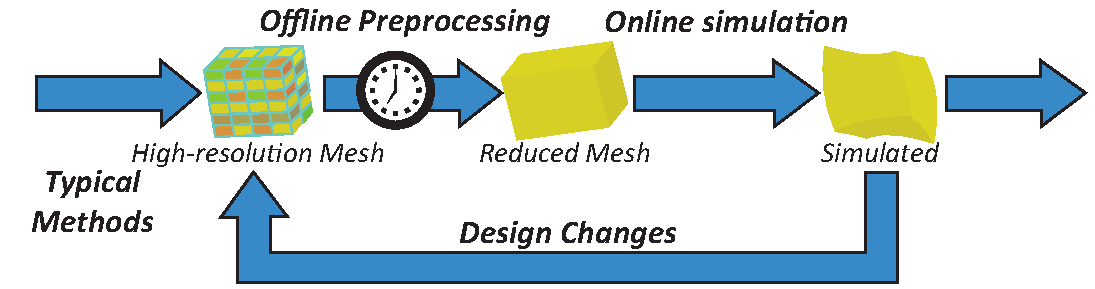
\includegraphics[width=0.8\textwidth]{figs/typical1.pdf}
	\caption{(a) In a typical method, the preprocessing step is offline,
		making the design loop slow. (b) In our method, we move the timeconsuming
		offline computation outside of the design loop.}
	\label{fig:typical}
\end{figure}

We propose Data-Driven FEM (DDFEM), a new simulation methodology
that removes these limitations and is thus extremely well suited
to the types of design problems discussed above.
We divide an object into a set of deformable voxels using embedded finite
elements and coarsen these voxels hierarchically.
A custom metamaterial database is populated with materials that minimize the error incurred by coarsening.
This database is learned once in a completely offline fashion and depends only on the set of materials to be used by the deformable object and not on the actual material distribution
and geometry.
At runtime we use the database to perform fast coarsening of an FEM mesh in a way that is agnostic to changes in geometry and material composition of the object.
The key features of the algorithm are its ability to handle arbitrary, nonlinear elastic
constitutive models as well as to avoid expensive precomputation
within the design loop (Figure~\ref{fig:typical}b).
DDFEM is the first algorithm optimized for interactive design of non-linear elastic objects.

\subsection{Overview}
DDFEM is a combination of embedded finite elements and hierarchical
coarsening.
In this section, we discuss the problem of coarsening
and introduce the notion of a material palette. We conclude by
summarizing the two main stages of DDFEM—offline metamaterial
construction and online coarsening.
\paragraph{Coarsening for finite elements}
The key component of our DDFEM is coarsening.
Coarsening reduces the number of vertices in a finite element simulation mesh in order to improve
runtime performance.
Since simply removing vertices can greatly reduce
the accuracy of the simulation, coarsening schemes also assign
new materials to coarsened elements to minimize this effect.
We regard the global coarsening of a simulation mesh as the result
of many local coarsening operations which map from contiguous
subsets of fine elements with applied materials to coarse elements
with new, optimized materials. Our goal is to precompute these
optimized materials so that coarsening is fast at runtime. Below we
discuss how to make such a precomputation tractable beginning with
our choice of Finite Element simulation methodology.
\paragraph{Conforming vs. embedded finite elements}
The defining feature of conforming finite element methods is that the simulation
mesh is aligned with the geometry of the object being simulated.
One obvious feature of conforming meshes is that the mesh itself is a
function of the input geometry.
This means that the output of a local coarsening operator (the coarsened mesh) will also be a function
of the input geometry.
Also, the new material computed by each local coarsening operator will be a function of input geometry.
This dependence on input geometry is a significant issue to overcome
if we wish to precompute coarsened materials because, in design
problems, the input geometry is in constant flux.
The number of precomputed coarse materials now depends on the local material
assignment on the simulation mesh and the input geometry.
Thus space of coarsened materials is prohibitively large.
To mitigate this we turn to embedded finite elements.
These methods embed the geometry to be simulated into the simulation mesh with no regard
for whether the mesh conforms to the geometry or not.
Thus an identical simulation mesh can be used for any input geometry.
Local coarsening operations on the embedded mesh yield identical coarse
elements and the optimized coarse material depends only on the
local material distribution on the simulation mesh. This significantly
reduces the size of the coarsened material space. In this paper we
embed all simulation geometry into a hexahedral simulation mesh.
\paragraph{Material palette} We further shrink the space of coarsening operators
using an observation about material design. Designers do
not work in a continuous space of materials but limit themselves to
a relatively compact set (e.g. rubber, wood, steel) related to their
problem domain. We call these discrete sets of materials
palettes and denote them $\mathcal{P}=\{\mathcal{M}^1,...,\mathcal{M}^n\}$.
Here $\mathcal{M}^i$ denotes a specific material model in $\mathcal{P}$, 
and $n$ is the size of the material palette.
In this work we limit ourselves to nonlinear hyper-elastic materials,
which means that each $\mathcal{M}^i$ can be represented by a strain
energy density function.
We also include a void (or empty) material in every palette.
This allows us to perform topology changes in the
same manner in which we perform material assignment updates.
\paragraph{Algorithms}
With the material palette in hand, we can now define our algorithm, which is divided into two distinct phases: an \textbf{offline database construction} stage and an \textbf{online coarsening} stage.  Below we detail the input, output, and steps of each stage:
\vspace{1mm}
\hrule
\textbf{Offline Database Construction}
\vspace{1mm}
\hrule
\begin{compactitem}
	\item \textbf{INPUT:} A palette of materials to be applied to high-resolution hexahedral simulation meshes $\set{P}^0$
	\item \textbf{OUTPUT:} A new palette of coarse metamaterials, $\set{P}^1$, and a mapping from fine material combinations to the coarsened materials in $\set{P}^1$. 
	\item \textbf{STEPS:}
	\item \textbf{FOR EACH} material combination applied to a 2$\times$2$\times$2 cube of high resolution elements
	\subitem $\bullet$ Sample potential energy function of 2$\times$2$\times$2 block
	\subitem $\bullet$ Fit metamaterial for coarse hexahedral element
	\subitem $\bullet$ Add metamaterial to $\set{P}^1$ using high resolution 
	\subitem material IDs as database key
	\item \textbf{END}
\end{compactitem}
\vspace{1mm}
\hrule
\vspace{1mm}
\hrule
\textbf{Online Coarsening}
\vspace{1mm}
\hrule
\begin{compactitem}
	\item \textbf{INPUT:} High resolution hexahedral simulation mesh with 
	\subitem material IDs and
	\subitem coarsened hexahedral simulation mesh 
	\item \textbf{OUTPUT:} Metamaterial assignments for coarse mesh
	\item \textbf{STEPS:}
	\item \textbf{FOR EACH} 2$\times$2$\times$2 block in the high resolution mesh
	\subitem $\bullet$ Replace with single coarse element
	\subitem $\bullet$ Assign material from $\set{P}^1$ using high resolution 
	\subitem material IDs as database key 
	\item \textbf{END}
\end{compactitem}
\vspace{1mm}
\hrule

\paragraph{Hierarchical coarsening}
We stress that both stages of the DDFEM algorithm can be applied hierarchically. Given the first level of metamaterials, $\set{P}^1$, we can construct a metamaterial library, $\set{P}^2$, for the second level by using $\set{P}^1$ as an input material palette. At runtime, the coarsening algorithm looks up materials from $\set{P}^2$ to replace each 2$\times$2$\times$2 coarse block with a single element.

Having introduced the broad strokes of the DDFEM scheme, we move on to a detailed explanation of each algorithmic component. First we discuss database construction, followed by the runtime component. We end by demonstrating the speed and accuracy of DDFEM.
\subsection{title}
\section{Metamaterial Database Construction}
\label{sec:database}
We construct our metamaterial database using a potential energy fitting approach. This is valid due to the hyperelastic materials that make up our material palettes. Material fitting considers 2$\times$2$\times$2 blocks of high-resolution hexahedral elements (denoted $^0\set{E}$). For each element $^0E_k\in \, ^0\set{E}$, its material is referred to as $^0\set{M}_k\in \, ^0\set{P}$. (Note that $\set{E}$ refers to a set of elements and $E$ refers to a single element.) Given $^0\set{E}$, we can sample its deformation space, and using $^0\set{M}_k$, compute the potential energy $^0V$ for each sample.  Now we must find a metamaterial that, when applied to a single coarse element $^1\mathit{E}$ best approximates $^0V$.  This is accomplished by fitting a metamaterial potential energy function , $^1V$, to the set of deformation/energy samples. The fitted metamaterial is stored in the metamaterial database and indexed by the material indices of $^0\set{M}$.

\subsection{Metamaterial Model}
Our fitting approach depends on choosing a good metamaterial model.
In order to ensure that our model meets the criteria for a material energy function~\cite{Marsden2012}, we choose our metamaterial model for $^1\mathit{E}$ as a combination of material models of $^0\set{M}_k$:
\begin{align}
^1V(^1\vr{u}, \, ^1\vr{p}) = \sum_{k=1}^8 w_k \, ^0V_k(^0\vr{u}_k, \, ^1\vr{p}_k, \, ^1\vr{X}_k),
\label{eq:materialModel}
\end{align}
where $^0V_k$ is the strain energy density of $^0\set{M}_k$ at quadrature point position $^1\vr{X}_k$ (\autoref{fig:coarseFine}). Here $^1\vr{u}$ is the vector of nodal displacements associated with $^1\mathit{E}$ while $^0\vr{u}_k$ are displacements for the $k^{th}$ element at level $0$ reconstructed using trilinear interpolation from $^1\vr{u}$. The vector $^1\vr{p}$ stores the material parameters for the coarse metamaterial and consists of the stacked material parameter vectors for each material in $^0\set{M}_k$, themselves denoted by $^1\vr{p}_k$.  $w_k$ is the standard Gaussian quadrature weight.
We note that our model incurs slight computational overhead at runtime because we must evaluate potential energy functions at 8 quadrature points.
%However, because each constituent material model can be evaluated independently, much of this deficit can be made up by parallelizing the computation.
%Furthermore
However, the speed improvement gained by coarsening makes the remaining, per-quadrature point expense negligible.

\begin{figure}
	\centering
	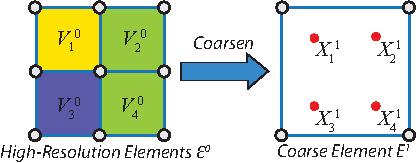
\includegraphics[width=0.6\textwidth]{images/coarseFine.pdf}
	\caption{The relationship between high-resolution and coarsened elements. At each quadrature point $^1\vr{X}_k$, the coarse element copies the corresponding energy density function $^0V_k$ from the high-resolution element.}
	\label{fig:coarseFine}
\end{figure}

We observe that even if the individual base material models are isotropic, the metamaterial can become anisotropic by assigning different material parameters at the quadrature points. We counter this by augmenting the metamaterial model with an anisotropic term, which improves fitting.
The complete model is then given by
\begin{align}
\begin{split}
^1V(^1\vr{u}, \, ^1\vr{p}, \, C) &= \sum_{k=1}^8 \bigg( w_k \, ^0V_k(^0\vr{u}, \, ^1\vr{p}_k, \, ^1\vr{X}_k)\\
& + C_k\left( \sqrt{\vr{v}^T\vr{F}_k^T\vr{F}_k\vr{v}} - 1\right)^2\bigg),\\
\label{eq:materialModel2}
\end{split}
\end{align}
where $\vr{v}$ is a unit-length direction of anisotropy and $C_k$ is the scaling parameter at the $k^{th}$ quadrature point. 

\subsection{Force Space Sampling}
\label{sec:force_space_sampling}
As mentioned previously, we take a sampling-based approach to metamaterial fitting. In order to fit our model (\autoref{eq:materialModel2}) to $^0V$ we first draw a number of samples from the deformation space of $^0\set{E}$ and compute $^0V$ for each sample.
If a user has prior knowledge of the set of meshes and simulations that they will require, then the best way to draw the samples is to run a number of anticipated simulations with various material combinations.
In this paper, we provide a more general method to draw samples for a metamaterial.
Initially, we attempted sampling by applying a random deformation to the corners of $^1\mathit{E}$; however, this led to many infeasible samples for very stiff materials.
In order to alleviate this problem we perform sampling in the force space.

For each element $^0\mathit{E}\in \, ^0\set{E}$ we apply a set of randomly generated forces.
We solve an elastostatic problem to compute the deformation of $^0\set{E}$, using constraints to remove rigid motion. Recall that this is fast because $^0\set{E}$ consists of just 8 elements.
Each sample is then a tuple $\left\{^0\vr{u}, \, ^0V\right\}$ (\autoref{fig:sampling}) where $^0\vr{u}$ are the nodal displacements of $^0\set{E}$, and $^0V$ is the strain energy density value of this deformed configuration.
\begin{figure}
	\centering
	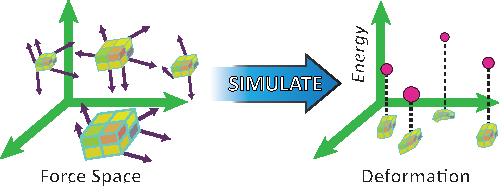
\includegraphics[width=0.8\columnwidth]{images/sampling.pdf}
	\caption{ We sample the energy function of a 2$\times$2$\times$2 block of hexahedra by applying random forces and deforming the block using FEM. Each set of forces results in a deformation-energy tuple which is used during fitting.}
	\label{fig:sampling}
\end{figure}

\subsection{Fitting}
\label{sec:fitting}
Given a set of deformation samples, $\left\{ ^0\vr{u}, \, ^0V\right\}$, we perform a least squares fit to determine the parameters, $^1\vr{p}$, for a given metamaterial (\autoref{fig:fitting}):
\begin{align}
^{1}\vr{p}^*= \underset{^1\vr{p}}{\operatorname{argmin}} \, \sum_{s=1}^{n_s}\left(^0V_s- \, ^1V\left(\vr{r}\left(^0\vr{u}_s\right), \, ^1\vr{p}\right)\right)^2,
\label{eq:fitting}
\end{align}
where $\vr{r}$ constructs $^1\vr{u}$ from $^0\vr{u}$, $n_s$ is the total number of samples, and $s$ indexes all samples. In our experiments we use the simplest form of $\vr{r}$ choosing it to extract the displacements of the corners of $^0\set{E}$.

\paragraph{Fitting in the Presence of Anisotropy}
If performed naively this optimization is nonlinear because we must simultaneously solve for $\vr{v}_k$, the preferred direction of anisotropy. This can severely slow the fitting procedure, especially in cases where it would otherwise be a linear least squares problem (i.e if all fine-scale materials are Neo-Hookean or a similarly simple material model).
To avoid this problem we first estimate all anisotropy directions, and then solve \autoref{eq:fitting} for the remaining material parameters.
Our intuition is that anisotropy manifests itself as preferential stretching along a particular axis. To find this axis, we apply stretching forces to a block in a discrete set of directions uniformly sampled over a sphere.
If the stretching force is close to the direction of anisotropy, then the amount of stretching deformation is reduced.
For any given stretching direction $\mathbf{v}$, we apply a stretching force and compute the deformation gradient $\mathbf{F}$ of  each quadrature point.
Under $\mathbf{F}$, a unit length vector in direction $\mathbf{v}$ is stretched to a new length $l = \|\mathbf{F}\mathbf{v}\|$.
The set of all 3D vectors $l\mathbf{v}$ forms an ellipse-like shape.
We find the principal axes of the ellipse (via SVD) and use them as directions of anisotropy.
\begin{figure}
	\centering
	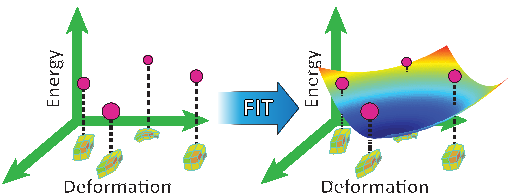
\includegraphics[width=0.8\columnwidth]{images/fitting.pdf}
	\caption{ Metamaterial potential energy functions are fitted to the deformation-energy samples using a least-squares optimization.}
	\label{fig:fitting}
\end{figure}
\paragraph{Regularization} Since vastly different material assignments, $^0\set{M}_k$, can produce the same metamaterial, our na\"{i}ve cost function (\autoref{eq:fitting}) can produce very large parameter values and even non-physical negative ones.
For example, consider a homogeneous material assignment at the high-resolution level.
The same metamaterial can be achieved by interleaving hard and soft materials at each fine element or by assigning a single, well chosen material to all fine elements.
To overcome this, we add a regularization term to control the parameter ranges and prevent overfitting of the training samples.
Our modified error function takes the following form:
\begin{equation}
\sum_{s=1}^{n_s}\left(^0V_s- \, ^1V\left(\vr{r}\left(^0\vr{u}_s\right), \, ^1\vr{p}\right)\right)^2 + 
\lambda\sum_k (^1\vr{p}_k - \, ^0\vr{p}_k)^2,
\end{equation}
which prevents material parameters from deviating too far from  $^0\set{M}_k$.
We chose the regularization constant $\lambda=0.02$ for the results in this paper.
In our experiments, since the base energy functions are linear with respect to the material parameters, the fitting problem can be solved by linear regression with regularization.

\begin{figure}
	\centering
	\includegraphics[width=0.8\columnwidth]{images/compression}
	\caption{Database compression step adds metamaterials to a compressed database by a farthest point sampling strategy.}
	\label{fig:compression}
\end{figure}

\subsection{Database Compression}
\label{sec:compression}
Given $n$ materials in the palette, the number of material combinations in a 2$\times$2$\times$2 block is $n^8$. In modern hardware, it is impossible to compute and store all material combinations even for a moderately-sized palette with $100$ materials.
In order to compress the number of materials stored in our metamaterial database, we select a small number of representative material combinations and remove all others. We compare materials in a feature space. In order to construct metamaterial feature vectors, we first select a common subset of deformations from all computed deformation samples. We then evaluate the potential energies of each metamaterial at each deformation sample. The stacked vector of energies becomes a metamaterial feature vector. 

Since our base materials differ in stiffness by orders of magnitude, we take the logarithm to measure the difference in ratio.
Let $D$ be the $L^2$ norm of log-energies between the two materials given by
\begin{equation}
D(A,B)=\sqrt{\sum_s (\log(^0V^{A}_{s})-\log(^0V^{B}_{s}))^2},
\end{equation} where $A$ and $B$ denote two distinct metamaterials in the database. 
Given the distance metric, we can select $k$ representatives materials using farthest point sampling~\cite{eldar1997farthest}. We randomly choose an initial metamaterial and then repeatedly select the material combination furthest away from any previous representatives -- continuing until we obtain $k$ representatives (\autoref{fig:compression}). This compression algorithm chooses $k$ samples that equally cover the metamaterial energy space, helping to preserve good behavior in our coarse simulations. 
\subsection{Hierarchical Coarsening}
While one level of coarsening can yield significant speed-ups, DDFEM can also be applied hierarchically.
As discussed in~\autoref{sec:compression}, the exponential growth of metamaterials palettes at each level makes it prohibitively expensive to perform fitting.
We address this by changing our coarsening strategy. 
Instead of choosing $^0\set{E}$ to be a 2$\times$2$\times$2 block we choose it to be a 2$\times$1$\times$1 block, which we coarsen. We construct an intermediate database of materials and compress. 
We then choose $^0\set{E}$ to be a 1$\times$2$\times$1 block, coarsen and compress, and finally a 1$\times$1$\times$2 block, coarsen and compress. Intermediate compression greatly reduces the number of samples we need to generate in order to populate the material parameter database for the next coarsening level. 
It is important to note that our intermediate databases only store lookup tables which allow us to extract appropriate material IDs for the next coarsening stage. Material parameters need only be stored in the final database since it is these elements that are simulated.
\begin{figure}
	\centering
	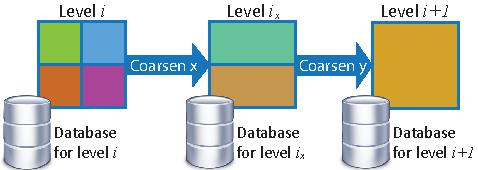
\includegraphics[width=0.7\textwidth]{images/hierchical}
	\caption{Hierarchical coarsening operates on one dimension at a time, performing clustering at each intermediate stage (here denoted $i_x$). This allows our compression algorithm to be applied aggressively, greatly reducing the number of energy samples we need for fitting material parameters. }
	\label{fig:hierarchy}
\end{figure}
\section{Runtime Simulation}
\label{sec:runtime}
Once our metamaterial database, $\set{P}^1$, has been constructed we can use it to perform fast online coarsening. 
Initially, the user loads geometry which is embedded in a hexahedral grid for simulation. Prior to simulation we iterate over all 2$\times$2$\times$2 blocks of hexahedral elements and perform mesh coarsening by replacing these 8 elements with a single coarse element. We perform a database lookup into $^1\set{P}$, using the material ID numbers of the 8 original elements, to quickly retrieve the optimal metamaterial for this coarse element. Database lookup is fast (even using our unoptimized, single-threaded implementation), and this is what makes DDFEM so appealing.
We achieve significant simulation speed-up from coarsening, retain accuracy in the simulation, and reduce the cost of material coarsening at runtime to a negligible amount.
	Our material model can be used in any simulation algorithm suitable for non-linear elasticity. In our experiments, we use Coin-IpOpt~\cite{ipopt} to implement static and dynamics simulations with tolerance (``tol'' option) set to $0.5$. We use Pardiso as our linear solver.
	For timing purposes, we limit Pardiso to single thread mode.
	The pseudo-code for static simulation is shown in \autoref{alg:sim}.
\begin{algorithm}[!h]
	
	\caption{Static Simulation}\label{alg:sim}
	\begin{algorithmic}[1]
		\REPEAT
		\STATE $\mathbf{f}$: global force vector
		\STATE $L$: triplet list for global stiffness matrix
		\FOR{each element e}
		\STATE compute elastic force $\mathbf{f}_e$
		\STATE add $\mathbf{f}_e$ to $\mathbf{f}$
		\ENDFOR
		\STATE add external force $\mathbf{f}_{ext}$ to $\mathbf{f}$
		\FOR{each element e}
		\STATE $\mathbf{K}_e$: element stiffness matrix
		\FOR{each quadrature point q}
		\STATE compute stiffness matrix $\mathbf{K}_q$ at quadrature point
		\STATE $\mathbf{K}_e+=\mathbf{K}_q$
		\ENDFOR
		\STATE append entries of $\mathbf{K}_e$ to $L$
		\ENDFOR
		\STATE sort $L$ to get sparse stiffness matrix $\mathbf{K}$
		\STATE set entries in $\mathbf{K}$ and $\mathbf{f}$ for fixed vertices
		\STATE $\Delta\mathbf{x}=\mathbf{K}^{-1}\mathbf{f}$
		\STATE compute step size $h$ using line-search
		\STATE $\mathbf{x}+=h\Delta\mathbf{x}$
		\UNTIL{convergence}
	\end{algorithmic}
\end{algorithm}
\chapter{Computation Design with Microstructures}
Many engineering problems focus on the design of complex structures that needs to meet high level objectives such as the capability to support localized stresses, optimal tradeoffs between compliance and mass, minimal deformation under thermal changes, etc. One very popular approach to design such structures is topology optimization.
Topology optimization generally refers to discretizing the object of interest into small elements and optimizing the material distribution over these elements in such a way that the functional goals are satisfied \cite{bendsoe2004topology}. Traditionally, topology optimization focused on designs made of homogeneous materials and was concerned with macroscopic changes in the object geometry.
With the advent of multi-material 3D printing techniques, it is now possible to play with materials at a much higher resolution, allowing to obtain much finer designs and, thus, improved functional performances.
Unfortunately, standard techniques for topology optimization do not scale well and they cannot be run on objects with billions of voxels. This is because the number of variables to optimize increases linearly with the number of cells in the object. Since many current 3D printers have a resolution of 600DPI or more, a one billion voxel design occupies only a 1.67 inch cube.

Most previous algorithms working in the material space focused on optimizing a single material property such as density or material stiffness, for which analytical formulas describing the property bounds exist \cite{Allaire93Bounds}. On the contrary, optimizing the structure and material distribution of an object in a high dimensional material property space remains an open problem. In this work, we propose a new computational framework for topology optimization with microstructures that supports design spaces of multiple dimensions. We start by computing the gamut of the material properties of the microstructures by alternating stochastic sampling and continuous optimization. This gives us a {\it discrete} representation of the set of achievable material properties, from which we can construct a {\it continuous} gamut representation using a level set field. We then reformulate the topology optimization problem in the continuous space of material properties and propose an efficient optimization scheme that finds the optimized distributions of multiple material properties simultaneously inside the gamut.
Finally, in order to obtain fabricable designs, we map the optimal material properties back to discrete microstructures from our database.

Our general formulation can be applied to a large variety of problems. We demonstrate its efficacy by designing and optimizing objects in different material spaces using isotropic, cubic and orthotropic materials. We apply our algorithm to various design problems dealing with diverse functional objectives such as minimal compliance and target strain distribution. Furthermore, our approach utilizes the high-resolution of current 3D printers by supporting designs with trillions of voxels. We fabricate several of our designs, thus, demonstrating the practicality of our approach.

The main contributions of our work can be summarized as follows:
\begin{itemize}
	\item We present a fully automatic method for computing the space of material properties achievable by microstructures made of a given set of base materials.
	\item We propose a generic and efficient topology optimization algorithm capable of handling objects with a trillion voxels. The key of our approach is a reformulation of the problem to work directly on continuous variables representing the material properties of microstructures. This allows us to cast topology optimization as a reasonably sized constrained optimization problem that can be efficiently solved with state of the art solvers.
	\item We validate our method on a set of test cases and demonstrate its versatility by applying it to various design problems of practical interest.
\end{itemize}
\section{Overview}
Given as input a set of base materials, an object layout, and functional objectives, the goal of our system is to compute the material distribution inside the object in order to optimize these functional objectives. In our approach, we do not solve the problem directly, instead we work with microstructures made of the base materials and the space of physical material properties spanned by them. The complete pipeline of our system, illustrated in Figure \ref{fig:overview}, can be decomposed into three stages.

\paragraph{Material Space Precomputation}
In the first stage, we estimate the gamut of material properties covered by all possible microstructures made by spatial arrangement of base materials. 
Since exhaustively computing the properties of all these microstructures is, in practice, intractable, we progressively increase the material space by alternating a stochastic search and a continuous optimization. The first step introduces discrete changes in the materials of the microstructures and allows emergence of new types of microstructures. The second step allows to locally push the material space boundaries by refining the microstructure shapes. After completing this stage, we obtain a discrete representation of the space of material properties and the mapping between these properties and the corresponding microstructures.

\paragraph{Gamut-based Continuous Topology Optimization}
In the second stage, we construct a smooth continuous gamut representation of the material property space by using a level set field. We define our topology optimization problem directly in this space. Our approach minimizes the objective function over possible material parameters while asking for strict satisfaction of the physics constraints -- typically, the static equilibrium -- as well as the strict satisfaction of the physical parameter bounds. Taking advantage of our gamut representation as a level set, we formulate this last constraint as limiting the material properties to stay on the negative side of the level set. This guarantees that the material properties that we use in the optimization are always physically realizable.

\paragraph{Fabrication-oriented Microstructure Mapping}
In the last stage, we generate a printable result by replacing each cell in the object layout with a microstructure whose material properties are the closest to the continuous material assignment resulting from the optimization. We also take into account the boundary similarity across adjacent cell interfaces to improve the connectivity between microstructures. This results in a complex, high-resolution, multi-material model with optimized functional specifications.
\section{Discovery of Extremal Microstructure Families}
Microstructures can exhibit remarkable physical properties that extend beyond the properties of their constituent materials. Many microstructure types have been developed to demonstrate applications in mechanics1-4, acoustics5,6, and electromagnetics7,8. These microstructures are typically designed by domain experts using time and labor intensive manual processes. These designs are often programmable in the sense that they have a small number of parameters to generate a family of geometries. A given microstructure family can be tested by performing simulations or experimental measurements on a set of samples drawn from it. The mapping between parameters and physical properties discovered in this testing process helps uncover the underlying design principles that drive these correspondences. In practical applications, mapping the parameter space also allows for the selection of a family member that has a desired tradeoff of physical properties9. Unfortunately, it is rare for manually designed microstructure families to reach extremal properties. This is because the space of possible microstructure designs is combinatorial and therefore impossible to explore exhaustively. One common approach to bypass this design challenge is to use computational methods, such as topology optimization10,11, with a computer simulation in their inner loop to find a microstructure with a desired tradeoff of physical properties. Unfortunately, constructing parametric models from these optimized structures has heretofore required further expertise and manual design effort12. In contrast to previous work, we present the first computational method to automatically explore the space of microstructure designs and discover parametric families optimized for competing properties.

While our methodology is not limited to specific physical properties, this study applied our method to design of mechanical microstructures. Specifically, we set our algorithm to search for a particularly interesting type of mechanical microstructures: auxetic materials, which have a negative Poisson��s ratio. These materials have the unusual property of becoming laterally thinner under axial compression. 2D auxetic structures are well understood due to their relatively simple geometry such as reentrant structures9, 13, chiral structures14, 15 and rotating mechanisms16,17. Generalizing existing 2D structures to 3D is challenging since a naive arrangement of 2D mechanisms often results in orthotropic or other anisotropic structures with low shear resistance. Such structures will prefer shearing deformation when the load is not aligned well with the auxetic direction. Additionally, since Poisson��s ratio for orthotropic structures is unbounded, orthotropic auxetic structures are much easier to find than isotropic ones18. Lakes fabricated and tested the first isotropic 3D auxetic structure13. However, designing manufacturable 3D auxetic structures remains a challenging task due to its complexity. Only a handful of 3D design patterns have been fabricated and measured18, 19. This study led to the discovery of five families with negative Poisson��s ratio and tunable shear resistance.

Our discovery pipeline has four steps (Fig. 1). The first step estimates the material property gamut, which is the range of material properties achievable by the microstructures. Here a microstructure is defined on a 3D regular grid composed of hexahedral voxels. The design space includes all possible material assignments to the voxels. Since exhaustively simulating all possible microstructures is impractical, this step computes a set of sample microstructures. The sampling algorithm alternates between topology optimization and stochastic discrete search to progressively expand the gamut20. The topology optimization stage pushes structures past the explored gamut boundary along gradient directions. The stochastic stage introduces discrete changes to escape local optima.

In the second step, common geometric traits are identified among microstructures near the gamut boundary. Geometrically similar structures are grouped into families using nonlinear dimensionality reduction (NLDR). Isomap21 is used as the reduction method because it can discover long sequences of related structures while keeping distant points separated. The effectiveness of NLDR depends on the distance metric that measures geometric difference. A smoothed Euclidean norm is chosen for robustness (Supplementary Fig. 1). NLDR outputs an embedding of the microstructures in a low-dimensional space where similar structures are closely packed. Microstructures in the embedding space are clustered using a Gaussian mixture model22 where each cluster corresponds to a family. Families with a significant number ($>200$) of members are extracted for further analysis.

The third step in our process constructs templates for each microstructure family. We observe that most of the extremal structures are composed from beams, plates and blocks. All of these structures can be represented as cuboids with different edge lengths. We therefore chose cuboids as the building blocks for microstructure templates, and note that some structures near the boundary do not fit the cuboid representation (Supplementary Fig. 4). To find a template from a family representative, its topology is computed using a morphological skeleton23. The morphological skeleton is a set of connected edges that largely preserves topological and branching characteristics of the structures. The skeleton is converted into a graph in order to represent a template. A cuboid is placed on each edge of the graph with optimized sizing and orientation to best match the representative structure. More details of the process are available in the supplementary text.

Finally, reduced parameters are computed to allow an intuitive navigation in the material property space. Since the templates from the previous step contain tens of parameters that do not directly correspond to material properties, it is still difficult to understand the key design principles. The reduced parameters allow for direct tuning of each material property. For a given parametric template, its parameters are fitted to all structures of the corresponding family. To avoid outliers, microstructures leading to large fitting errors ($>5\%$ voxel difference) are excluded. Principal component regression (PCR) is then performed on the set of fitted template parameters to find principal directions in the template parameters space. Varying the parameters in a direction corresponds to moving on the gamut boundary in a certain direction. A reduced parameter is assigned to each direction to control amount of change along that direction.
\subsection{Results and Discussion}
The results of this study focus on elastic material properties: Young��s modulus, Poisson��s ratio and shear modulus. The elastic material property gamut is estimated from 15,000 3D cubic-symmetric microstructures at a voxel resolution of 643. The voxel resolution is a power of 2 because that is necessary to achieve optimal performance of our multigrid FEM simulation. The specific resolution 643 is chosen because it is sufficient for discovering auxetic structures with a wide range of relative shear modulus while 323 structures cannot achieve comparable complexity or property ranges. The macroscopic elastic parameter of each microstructure is computed using homogenization theory24, 25 assuming a periodic boundary condition, (i.e. the structure is repeated infinitely). Each microstructure consists of a per-voxel binary material assignment. Due to manufacturing limits on minimum feature size, sensitivity filter26 is applied in gamut sampling step to avoid structures with overly thin features.

Here we focus on analysis of auxetic structures since families with positive Poisson��s ratios are relatively simple (Supplementary Fig. 2). Five families with significant number of members (Fig. 2b) are discovered using three Isomap embedding dimensions. We confirmed that Isomap associates seemingly distant structures through intermediate structures. For example, structures 5-1 and 5-3 from family 5 have very different beam thicknesses resulting in large geometric distance. However, the embedding reveals that there is a sequence of structures such as 5-2 that make the connection between them.

For each of the five families, a parametric template is automatically constructed. The initial topology of a template is extracted from the morphological skeleton of a representative structure (Fig. 3b). While the topologies are visually complex, they are generated by mirroring a small number of beams (highlighted in red) reflected according to cubic symmetry (Supplementary Table 2). The most complex template 5 contains only 6 control beams. The five families cover similar ranges of Young��s modulus and Poisson��s ratio. However, they span different ranges of shear modulus. Inspired by classical linear elasticity theory, we compare the shear modulus ratio defined as
,
where G is shear modulus, E is Young��s modulus and �� is Poisson��s ratio. For traditional isotropic materials, the theoretical ratio is one. A low ratio indicates low resistance to shear deformation. For auxetic materials, lower ratios are much easier to obtain than higher ones. Even with foam structures assumed to be isotropic, experimental data from previous work indicates that the ratio is less than one27.

Template 1 resembles the conceptual sketch by Lakes13 and belongs to the reentrant class of geometry. The difference is that our template has only two beams mirrored by cubic symmetry while Lakes�� sketch contains three (Supplementary Fig. 6). It is the simplest auxetic template that we identified, as our microstructure database does not contain any single-beam auxetic structure. The shear modulus ratio of this family falls in the range between 0.07 and 0.24, which is the lowest among all five families. Templates 2 and 3 are similar to each other and differ by a diagonal beam in the face center (highlighted in green in template 3). Since their geometric difference is small, they are adjacent in the Isomap embedding space. The central beam is responsible for increasing the shear modulus of the structures. For structures with �� around -0.5, the additional beam increases the maximum shear modulus ratio from 0.34 to 0.90. Templates 4 and 5 also differ by a single beam. Even the most complex template 5 is optimized from a simple cube frame through our continuous optimization step as shown in our supplemental material (Supplementary Video 1). The additional beam in template 5 makes the family stiffer overall. Both families can achieve shear modulus ratio greater 1 for ��<-0.5.

For each family, principal directions of template parameters are extracted using PCR. The templates and reduced parameters are included with the report. Two significant directions correspond to change in Young��s modulus and shear modulus are kept for tuning structures. These directions reveal that for families 2 and 3, the thickness of the slanted column (Fig. 4a highlighted in red) is crucial for Poisson��s ratio where the Poisson��s ratio increases quickly with increasing beam thickness. For families 4 and 5, the thickness of the rotating triangle (Fig. 4b) affects the tradeoff between Young��s modulus and shear modulus (Supplementary Fig. 5).

While our cuboid-based templates are very simple, they are sufficient for replicating the auxetic behavior of the corresponding families. We validated the auxetic properties of the fitted microstructures using simulation. New structures are generated by varying template parameters. 300 new structures are sampled from each family along two PCR coordinate directions. The coverage of the templates in the microstructure gamut (Fig. 2b) shows that the templates can generate microstructures on the gamut boundary 

So far all of our simulations are carried out assuming linear elasticity, which is only accurate for infinitesimal deformations. We also make the common assumption that there is no self-collision. This assumption also imposes a limit on the maximum compressive strain we can apply to our structures before self-collision occurs. Representative structures from Families 4 and 5 have the lowest limit at $7\%$ compressive strain.
In practice, non-linear deformations such as bending and rotation are prevalent in our auxetic structures. Such deformations can cause linear elasticity to incorrectly predict significant volume expansion of rotated parts (up to $20\%$ percent in our test cases).
Thus, we tested our structures using a nonlinear material model to understand their behavior under large deformations. We simulated nonlinear deformation behavior using Neo-Hookean material model28.
At maximum allowed strain of $7\%$, linear elasticity and Neo-Hookean model still has acceptable agreement with an average error of $16\%$ in computed Poisson��s ratio. In addition to simulation, we also printed three example structures from each family with varying Young��s modulus and material ratio. Our structures demonstrated consistent auxetic behavior (Supplementary Video 3) even though they are optimized with linear elasticity assumption. Our structures do not rely on structural instability29 for auxetic behavior and shrinks uniformly as load increases. This means that their deformations consistently follow the same pattern for different trials.

Our process automatically discovered two types of auxetic mechanisms: slanted columns and rotating triangles (Fig. 4). The slanted column mechanism transforms vertical compression to horizontal motions. The rotating triangles transform vertical compression into a winding deformation that pulls the right end of the mechanism towards the center of the microstructure. Their motions are shown in supplementary video S3. While rotating triangles bear resemblance to existing 2D structures30 known as chiral structures (Supplementary Fig. 6d), its extension to 3D cubic structure with large shear modulus has never before been constructed. Additionally, the entire mechanism is discovered entirely automatically without imposing any artificial design restrictions �C all microstructures are built from hexahedral voxels. To inspire future applications of these mechanisms, we report the loading behavior of the mechanisms. These auxetic mechanisms are the most active parts in the microstructures. They act like joints that connect the more rigid scaffolding in microstructures. Because of this, they undergo the most deformation and concentrate a large amount of stress. For the rotating triangles, the stress is concentrated on the connections around the triangle. We computed the maximum principal strain in the structure with respect to the vertical compressive loading to provide insights into the strength of the block.
At the maximal compressive loading $(7\%)$, the maximum principal strain in the structure is $7\%$. Calculation using a reported Young��s modulus of 80MPa yields a von Mises stress of 6.72MPa (Fig. 4e) while our print material has a reported strength of 8.5MPa. The printed structures are approaching the strength limit under the load. Since the available material is relatively weak even compared to common materials such as ABS plastics and rubber, we believe that structural strength can be improved significantly with future manufacturing materials.

We have shown a computational method that combines discrete sampling, continuous optimization and dimensionality reduction methods for automatic discovery of new microstructure families and mechanisms that would have been challenging to design manually.
The discovered structures are suitable for manufacturing as they avoid thin features and distribute deformation over beams instead. They also span a wide range of shear moduli, allowing engineers to balance between different macroscopic properties. While our case study focuses on elastic material properties, the technique may be applied to other physical properties whenever predictive simulation exists. Our computational pipeline paves the way to discovery of structures that balance mechanical, thermal, optical, acoustic and electromagnetic properties. Moreover, it advances the understanding of underlying mechanisms that are crucial to extremal properties.

\section{Topology Optimization}
\label{sec:topoOpt}
A classic topology optimization problem consists of optimizing the shape and structure of a given object defined by a prescribed domain in order to minimize some cost function. For example, the standard topology optimization minimizes the compliance of the object while satisfying the static equilibrium and the total weight constraint.
Since the topology of the object is unknown {\it a priori}, a method of choice is to define the shape of the object through its material distribution and to locally work with material densities. To this end, the design layout is voxelized and a density variable is assigned to every cell of the discretized domain. By penalizing intermediate values for these densities, a binary distribution corresponding to the object's final layout can be eventually obtained.

In this work, we extend the traditional topology optimization algorithm in multiple ways.
First, we do not compute a binary material distribution at the cell level as commonly done. 
Instead, we leverage our database of microstructures and ask for each cell to be filled with one of the microstructures.
By doing so we change the topology of the object at a finer scale, i.e. within each cell. This is done by working with the macro-scale material properties of the microstructures instead of their geometry directly. The second difference is that our algorithm can be used with parametrizations of the material property space that are more complex than the single density parameter per cell that is commonly used in the standard topology optimization algorithm. Indeed, in our generalized topology optimization problem, each cell $c_i$ contains an n-dimensional material parameter $\bp_i\in \mathcal{R}^n$. We use $\bp$ to denote the stacked vector of material parameters in all cells.
Given a signed distance function $\Phi(\bp_i)$ that defines the gamut,
our new topology optimization problem is then written as
\begin{equation}
\begin{aligned}
\min_{\bp} : \quad & \mathcal{S}(\bp,\mathbf{u}) & \\
s.t. : \quad & \mathcal{F}(\mathbf{\bp},\mathbf{u})=0 & \\
: \quad & \Phi(\bp_i)\leq 0,  \quad 1\leq i \leq N_c&	
\label{eq:op}
\end{aligned}
\end{equation}
where $\mathcal{S}$ is a real-valued objective function that depends on the material parameters and the displacement vector $\bu$ of the entire object at the elasticity equilibrium.
The equality constraint $\mathcal{F}=0$ requires $\bu$ to satisfy the elasticity equilibrium and the inequality constraint $\Phi\leq0$ guarantees that the material properties of each cell stay inside the precomputed gamut.

In our examples, the material parameter $\bp$ consists of the density $\rho$ and the elasticity parameters $\be$.
We split our objective function into an elasticity term $\mathcal{C}(\vect{e},\bf u)$ that controls the deformation behavior (see Section \ref{sec:obj}) and an optional density term $\mathcal{V}(\rho)$ that controls the overall mass of the object.The density term can be written as
\begin{equation}
\mathcal{V}(\rho)=(\sum_{i=1}^{N_c}\rho_iV_i-\hat{M})^2\label{eq:vol},
\end{equation}
where $V_i$ is the cell volume and $\hat{M}$ is the target overall mass.
When one of the base material is void, the use of the density term allows to modify the topology of the object at a larger scale than the one of the microstructures, and thus to change the external shape of the object. 
In fact, even for multi-material designs involving base materials with similar mass densities, we noted that we could use the density term to encourage the presence of soft material in the structure. By removing the external cells entirely made of the soft material, we could then decrease the mass of the structure without significantly changing its mechanical behaviour.
Alternatively, the density term can also be used to control other quantities related to the ratios of the different materials such as the cost of the object.
For specific problems, we can also add spatially-varying weight control terms to Equation \ref{eq:vol}.
For example, we can control the target weight of each individual cell by adding a local term $(\rho_i-\hat{\rho}_i)^2V_i$.

Assuming static equilibrium, the elasticity constraint is written as 
\begin{equation}
\mathcal{F}(\mathbf{e},\mathbf{u})=K(\mathbf{e})\mathbf{u}-\bf f_{ext}=0,
\end{equation}
where $\bf f_{ext}$ are the external loads applied to the object.

The gamut constraint for a point $\mathbf{p}_i$ in the material property space is described by an $n$-dimensional level set function $\Phi(\mathbf{p})$.
We have $\Phi(\mathbf{p}_i)<0$ for a point inside the gamut, $\Phi(\mathbf{p}_i)>0$ for a point outside the gamut, and $\Phi(\mathbf{p}_i)=0$ for a point on the boundary of the gamut.
The value of $\Phi$ represents the $n$-dimension Euclidean distance to the level set boundary. %This distance can be linearly interpolated from the precomputed signed distance field.
The gradient of $\Phi$ are evaluated by a finite difference operation on the signed distance field.

We used a standard gradient-based numerical optimizer (Ipopt~\citep{ipopt} in our implementation) to solve Equation \ref{eq:op}. We enforced the elasticity equilibrium constraint using the adjoint method. The optimizer only needs to take the function values of $\mathcal{S}$ and $\Phi$ along with their gradients as input.

\subsection{Elasticity Objectives}\label{sec:obj}
We used two different types of objective functions for the elasticity term in our topology optimization algorithm. These two types of objectives allowed us to design a wide range of objects.
\paragraph*{Target Deformation}\label{sec:strain}
Our algorithm takes a vector of nodal target displacements and boundary conditions (external forces, fixed points, etc.) as input. Then, it automatically optimizes the material distribution over the object domain to achieve the desired linear deformation assuming a linear elastic behavior.

We define the deformation objective as
\begin{equation}
\mathcal{C}_d(\mathbf{e},\mathbf{u})=(\mathbf{u}-\hat{\mathbf{u}})^T \bD (\mathbf{u}-\hat{\mathbf{u}}),\label{eq:td}
\end{equation}
where $\hat{\mathbf{u}}$ is the vector of the target displacements, $\bf D$ is a diagonal matrix that determines the importance of each nodal displacement.	
We use $\bf D$ to define the subset of nodes that we are interested in.
For example, we can set most entries of $\bf D$ to zero and focus on a portion of the domain (see Figure \ref{fig:gripper}).

\paragraph{Minimum Compliance}\label{sec:compliance}
We have experimented with the same objective as the one used in the standard topology optimization algorithm where the compliance $\mathcal{C}_c$ is defined as
\begin{equation}
\mathcal{C}_c(\mathbf{e},\mathbf{u})=\mathbf{u}^T \bK(\mathbf{e}) \mathbf{u}.
\label{eq:mc}
\end{equation}
In the commonly used SIMP algorithm, the stiffness matrix $\bK_i$ of each cell $i$ depends on the artificial density value $\rho_i$
through an analytical formula such as $\bK_i = \rho_i^3\bK_0$ where $\bK_0$ corresponds to the stiffness matrix of the base material.
In contrast, the stiffness matrix in our objective function is directly computed from the material parameters of the material space and forced to correspond to a realizable material thanks to our gamut constraints.

Like in standard algorithms, we regularized the problem to avoid checkerboard solutions by applying a smoothing kernel on the material properties that favors smooth variations of the material parameters over the object layout.
Our optimizer supports multiple objectives by linearly combining weighted objective functions.
\section{Mapping Material Properties to Microstructures}
\begin{wrapfigure}{r}{0.2\linewidth}
 	\makebox[\textwidth][l]{\hspace{-0.4cm} \includegraphics[width=1.0\linewidth]{images/TranslatedMicrostructureVertical.png}}
\end{wrapfigure}
After running the topology optimization algorithm, we generate a printable result by replacing each cell in the object lattice by a microstructure whose material properties match the optimal ones.

Material properties of the microstructures are computed using the homogenization theory which is more accurate with a smooth transition between the geometries of neighboring cells.
While smoothness in the material parameters can be easily enforced, it does not imply topological similarity of nearby microstructures. 
For example, any translation of a given microstructure in a periodic tiling will result in a microstructure geometrically different but with exactly the same mechanical properties. 
Fortunately, our database is very dense and multiple microstructures generally map to similar points in the material property space, offering several variants. To further increase the number of possibilities, we also incorporate an additional exemplar for each microstructure by translating it by half its size, which preserves its cubic or orthotropic symmetry without changing its properties (see inset Figure). We then run a simple but effective algorithm that picks the microstructure exemplars that minimize the boundary material mismatch across adjacent cells. We quantify this mismatch by $\mathcal{I}=\sum_{i=1}^{N_c} \mathcal{I}_i$, where $\mathcal{I}_i$ is the contribution associated to the cell $i$ and corresponds to the number of boundary voxels filled with materials that are different from the ones of the voxels' immediate neighbours across the interfaces.

Our algorithm proceeds as follows:
\begin{itemize}
\item For each cell, we define a list of possible candidates by picking all the microstructures mapping to material points lying in the vicinity of the optimal material point and we randomly initialize the cell with one of the candidates.
\item We compute the mismatch energy $\mathcal{I}_i$ associated to each cell $i$ and sort the cells according to their energy. 
\item We pick the first cell in the sorted list, i.e. the one with the highest energy and assign to it the microstructure candidate that decreases the energy the most. If we cannot decrease the cell energy, we move to the next cell in the list.
\item We update the mismatch energies of all the impacted cells and we update the priority list.
\item We repeat the last two steps until the mismatch energy $\mathcal{I}$ cannot be decreased anymore.
\end{itemize}

\section{Results and Discussion}
We first analyzed our microstructure sampling algorithm for 2D and 3D microstructure gamuts. Then we used these precomputed gamuts and we designed and optimized a wide variety of objects with our topology optimization algorithm.
\subsection{Microstructure Sampling}
We evaluated our method on two- and three-dimensional microstructures made of one or two materials. For the 2D case we considered patterns with cubic and orthotropic mechanical behaviors that can be described with 4 parameters (3 elasticity parameters and density) and 5 parameters (4 elasticity parameters and density) respectively. In 3D we computed the gamut corresponding to cubic structures with 4 parameters. In all cases, the size of the lattice for the microstructures was set to 16 in every dimension. We used isotropic base materials whose Young's modulus differed by a factor of 1000 and having 0.48 as Poisson's ratio. We initially computed the databases for two-material microstructures, but also adapted these databases for microstructures made of a void and a stiff material. In the later case, we replaced the softer material by void, filter out all the microstructures with disconnected components and, in the 3D case, filled the enclosed voids and recomputed the homogenized properties. We provide a comparison between the initial and postprocessed databases in the supplementary material. The resulting postprocessed gamuts are also depicted in Figure \ref{fig:gamuts}. 
Our databases contain 274k, 388k and 88k 2D cubic, 2D orthotropic and 3D cubic microstructures respectively and took from 15 hours to 93 hours to compute, which correspond to 68, 19 and 5 sampling cycles, respectively.
\begin{figure}
	\centering
	\includegraphics[width=.24\linewidth]{images/2D_cubic.png}
	\includegraphics[width=.24\linewidth]{images/2D_ortho.png} 
	\includegraphics[width=.24\linewidth]{images/3D_cubic.png}
	\includegraphics[width=.24\linewidth]{images/3D_cubic_Panetta.png}
	\caption{Gamuts computed with our discrete-continuous sampling scheme for 2D cubic structures (\emph{left}) , 2D orthotropic structures (\emph{second from left}), 3D cubic structures (\emph{second from right}) and 3D cubic structures with 0.35 as Poisson's ratio (\emph{right}). The plots show the results for the projection of the gamuts on the plane defined by the macroscale Young's modulus along the x axis (normalized by the Young's modulus of the stiffest base material) and the Poisson's ratio corresponding to a contraction along the y-direction when the material is stretched along the x-direction.
		The blue dots correspond to the generated samples,the orange dots correspond to the microstructures from~\citet{Schumacher:2015} and the yellow dots correspond to the microstructures from~\citet{Panetta:2015}.}
	\label{fig:gamuts}
\end{figure}
We first compared our results to the ones obtained by~\citet{Schumacher:2015}
and observed a significant increase in the coverage of the material space, even for 2D microstructures where we used a coarser discretization. This comforts us with the idea that topology optimization only, while helpful to locally improve the microstructure geometries, is suboptimal when one aims to discover the entire gamut of physical properties. The diversity of the microstructures that we obtained is also much richer, thus providing a larger set of options for the practical use of microstructures. Note that they employed some regularization to avoid thin features. For $16^3$ microstructures, we found regularization unnecessary since they are manifold and have a minimal feature size  of 1/16 of the lattice size, which is the same order of magnitude as the thinnest parts of Schumacher's microstructures.
For completeness, we also compared our database of 3D microstructures to the one of~\citet{Panetta:2015} at $16^3$ and $64^3$ grid resolutions (Figure \ref{fig:gamuts}, \emph{right}). Our initial database was computed with 0.48 as Poisson's ratio and is shown in the supplementary material. For this comparison, we then recomputed the material properties of the microstructures using the same Poisson's ratio as Panetta's, i.e 0.35, which affects the extremal values of the obtained gamut.
For the $64^3$ microstructures, we used morphological operations in the discrete step and sensitivity filtering with a radius of 3 voxels in the continuous step to limit the minimum feature size to 1/32 of the lattice size~\citep{sigmund:2007}. Note that this comparison is provided for reference only since our microstructures are cubic while Panetta's are isotropic (a subset of cubic). Furthermore, they target a different 3D printing technology with self-supporting constraints not imposed here.
Finally, we also obtained a dense sampling in the interior of the space, as a result of the randomness inherent to our approach. This reduces the need of running costly optimization in these areas and occurs even if we do not explicitly enforce any sampling there.

We also experimented with three-material 2D cubic microstructures (two solid materials with Young's moduli differing by a factor of 1000 and with 0.48 as Poisson's ratio, plus a void material). The resulting database contains about 800k microstructures that can potentially be printed. The corresponding gamut and some examples of the generated microstructures are shown in Figure \ref{fig:Cubic2D_3Materials}.
\begin{figure}
	\centering
	\includegraphics[width=.5\linewidth]{images/Cubic2D_3Materials.png}
	\caption{Gamut corresponding to 2D cubic microstructures made of two materials and void. The Young's modulus of the microstructures is plotted using a logarithmic scale. We show above some examples of microstructures lying near the estimated boundary of the gamut, i.e. with extreme material properties. The dark color corresponds to the softer material, while the light grey color is used for the stiffer material.}
	\label{fig:Cubic2D_3Materials}
\end{figure}
\subsection{Topology Optimization}
We tested our topology optimization algorithm on a number of simple test cases and large scale examples. Detailed analysis and discussion of the results is provided below.

\paragraph{Impact of the Material Space}
We evaluated the impact of the chosen material space on a 2D cantilever beam with optimized minimum compliance. We tested our topology optimization algorithm on isotropic, cubic and orthotropic gamuts as well as with the virtual materials used in the traditional SIMP approach and for which the stiffness of the material $E=\rho^p E_0$, $p \geq 1$ is a function of the density $\rho$ of the cell and the stiffness of the base material $E_0$. We also tested our algorithm on an analytical gamut with allowed stiffnesses $E$ defined by $E\leq \rho^3 E_0$. The results are shown in Figure \ref{fig:defo_cvg}. It can be noted that, as the dimension of the material space increases, the final energy of the system decreases. This is to be expected since higher dimensional space means larger gamuts.
Thus, when using cubic materials, the minimum compliance objective function reaches 3\% lower energy than the standard SIMP method with power index 3.
This difference reaches 11\% when we use orthotropic materials.
It is worth noting that the lowest elastic energy is achieved when we use the traditional SIMP method with $p=1$ (as shown in Figure \ref{plot:cvg}). However, this solution does not correspond to a realizable structure since some of the optimized materials do not correspond to any microstructure.
\begin{figure}
	\centering
	\includegraphics[width=0.95\textwidth]{images/cantilever.png}
	\caption{Material property distributions optimized in the orthotropic (\emph{top left}), cubic (\emph{bottom left}), isotropic (\emph{top middle}) and an analytically defined gamut $E \geq \rho^3 E_0$ (\emph{bottom middle}), with the material property space dimensions ranging from five to two. 
		We compare our algorithm with the standard SIMP method with power index $p=1$ (\emph{top right}) and $p=3$ (\emph{bottom right}). For these figures, we computed the color of each cell by mapping every base vector of the normalized parameter space to a color range and linearly interpolating the colors associated to each of the parameters.
		In this example, the left side of the cantilever is fixed while a force distribution is applied to the bottom side (see red arrows in the top left picture).}
	\label{fig:defo_cvg}
\end{figure}

\begin{figure}[h]
	\centering
	\includegraphics[width=0.95\textwidth]{figs/cvg_test.png}
	\caption{Convergence tests. Variation of the objective energy (\emph{left}) and the elastic energy \emph{right} of a beam being optimized for minimum compliance as the optimization progresses. The convergence plots correspond to the beam of Figure \ref{fig:defo_cvg} when optimized using different material spaces (\emph{top}), different resolutions for the beam lattice (\emph{middle}) when using cubic microstructures, and different initial material properties for the cubic microstructures (\emph{bottom}).}
	\label{plot:cvg}
\end{figure}
\begin{figure}
	\centering
	\includegraphics[width=.5\linewidth]{images/bar_visio_new.png}
	\caption{
		Optimizing a beam to take an ``S'' shape under compression.
		A beam with homogeneous material can only compress uniformly (left column).
		The optimized beam can deform as requested (right column).
		Target displacements are set on the horizontal boundary cells.
		The color plot for the bottom beams shows the deformation error of each cell defined by Equation~\ref{eq:td}.
		\label{fig:beam_S_shape}}
\end{figure}

\paragraph{Matching Quality}
	We evaluated for different examples the matching quality of the target deformation optimization.
	For the first test, we forced a beam to take an `S' shape when undergoing tensile forces (Figure \ref{fig:beam_S_shape}). In order to avoid overfitting, we applied target displacements on the vertices of the boundary cells only. As depicted in the figure, the use of microstructures largely improves the global shape of the beam, which closely matches the target deformed shape. This becomes even more striking when compared to the behavior of a beam made of a homogeneous material.
		We also validated our algorithm by designing a soft ray whose wings can flap using a compliant mechanism (see Figure \ref{fig:ray} and accompanying video). Boundary conditions are applied on two circular areas located along the spine of the ray. Each disk has one degree of freedom for deformation, namely contracting or expanding along the disk normals. This mechanism resembles the one of many hydraulics-driven soft robots. We define two target deformation objectives corresponding to the flapping of the wings up and down, when alternatively contracting and expanding the two disks' boundaries. By running our multi-objective topology optimization framework, we can compute an optimized material design that can achieve both deformation modes when the corresponding boundary conditions are exerted.

\begin{figure}[t]
	\centering
	\includegraphics[width=.6\linewidth]{images/ray.png}
	\caption{Designing a soft ray. The wings of the ray flap up and down when cells on its spine contract and expand.
	Constrained vertices are colored in green.
	The deformations achieved with the optimized materials are displayed on the bottom row.}
	\label{fig:ray}
\end{figure}
\paragraph{Convergence and Robustness}
We evaluated the convergence rate of our topology optimization both on the minimum compliance problem and with the target deformation objective. For the minimum compliance problem, we used the same loading as the one of Figure \ref{fig:defo_cvg}. The corresponding results are shown in Figure~\ref{plot:cvg} where we plot both the deformation energy of the structure as defined in Equation \ref{eq:mc} and the original objective of the problem \ref{eq:op} that also includes the volume term defined by Equation \ref{eq:vol}. For all these examples, the algorithm converged after a couple of dozen iterations, irrespectively of the lattice resolution, i.e. the number of variables and the number of non-linear constraints. This demonstrates the scalability of the our algorithm. We also tested the robustness of our algorithm by starting with different initial conditions. In this case, we initialized the material parameters of each cell with a random material point projected onto the boundary of the gamut. Similar to other topology optimization schemes, we have no guarantee that we reach the global minimum of the function, and indeed, our algorithm sometimes converges to different solutions. However we note that these different solutions have a similar final objective value and are therefore equally good.

For the evaluation of the target deformation optimization, we tested the convergence rate when optimizing for functional mechanisms.
To this end, we designed several grippers that can grasp objects by moving their tips when external forces are applied to their extremities. We experimented with four sets of boundary conditions, namely, pulling and pushing the back of the gripper horizontally, and compressing and stretching the extremities of the gripper vertically. As shown in Figure \ref{fig:gripper}, these different settings lead to different material structures. The deformation errors of all the four designs converge to a low level after a couple of hundreds of iterations.

\begin{figure}[t]
	\centering
	\includegraphics[width=0.9\linewidth]{images/gripperVar.png}
	\includegraphics[width=0.4\linewidth]{images/gripper4_L2.pdf}
	\includegraphics[width=0.4\linewidth]{images/gripper4_Linf.pdf}
	\caption{Designing functional grippers. The left column shows the rest shape of the gripper and the target deformation for the tip.
	The green dots correspond to the fixed vertices while the blue arrows are the target displacements.
	The middle and right columns correspond to the optimized results obtained for the specified boundary conditions.
	The inset pictures color-code the initial and final deformation error for the different examples.
	The convergence plots in the bottom row depict the change in the sum of the deformation errors corresponding to all the cells (left) and the value of the maximal cell error contribution (right) as the optimization progresses.}  
	\label{fig:gripper}
\end{figure}
\paragraph{Accuracy}
\begin{figure}
	\centering
	\includegraphics[width=.6\linewidth]{images/hom_beam.png}	
	\caption{Comparison of simulated beams with homogenized material properties (\emph{inset pictures}) to the ones using full microstructures (\emph{large pictures}).
		}\label{fig:hom_beam}
\end{figure}

\begin{figure}[h]
	\centering
	\includegraphics[width=.8\linewidth]{images/hom_cube_random.png}	
	\caption{Comparison of simulated cubes with different material patterns modeled by homogenized cells (\emph{inset pictures}) and full resolution microstructures (\emph{large pictures}).}
		\label{fig:hom_cube_2}
\end{figure}

We evaluated the accuracy of our algorithm on several optimized structures by comparing the deformation obtained when using the optimized homogenized material properties for each cell to the one obtained by a high resolution simulation in which every cell is replaced by its mapped microstructure.
We first evaluated the accuracy on a deformable bar, one side of which was rigidly attached while the other was subject to different sets of external conditions (see Figure \ref{fig:hom_beam}). We used a $8\times2\times2$ lattice to represent the bar with homogenized cells, which translates into a $128\times32\times32$ grid for the full resolution mesh. Similar stretching, bending and shearing behaviors were obtained for both sets of models. From a quantitative point of view, the differences amount to 5-10\% in terms of average vertex displacement and 9\%-33\% in terms of elastic deformation energy (see Table \ref{tab:hom}). We further evaluated the effects of material patterns by running a similar comparison on a cube made of periodic layers of similar microstructures and with random assignments of microstructures (Figure \ref{fig:hom_cube_2}).  As reported in Table \ref{tab:hom}, we show that the ratio between the magnitudes of the average vertex displacement differences is between 4\% and 7\%, and the elastic energy difference is between 10\% and 19\%.

Finally, we also compared the behaviors of one of the grippers (Figure \ref{fig:gripper_validate}). The original optimized gripper is made of 3k elements while the high resolution version is made of 4M voxels.
Overall, the two models exhibit similar global deformation behaviors, in particular in the tip area. Some differences can be observed on the left side of the gripper for which the high-resolution model exhibits a lower effective material stiffness than its homogenized counterpart. With the same displacement boundary conditions applied, the high-resolution model deforms about 25\% more than the homogenized model.
	
	\begin{figure}[t]
		\centering
		\includegraphics[width=.6\linewidth]{images/gripper_cmp.png}	
		\caption{Comparison of a simulated gripper with homogenized material properties (\emph{inset picture, left}) to the one using full microstructures (\emph{main picture, left}). The figures on the right show the vector field of vertex displacement of the two models. The blue-to-red colors represent the magnitudes of the displacements.}
			\label{fig:gripper_validate}
	\end{figure}
	
	\begin{figure}[h]
		\centering
		\includegraphics[width=.6\linewidth]{images/hom_cube_peri.png}	
		\caption{Simulation of a cube made of a periodic arrangement of a single microstructure at different resolutions. Inset pictures correspond to the model with homogenized material properties, while main pictures correspond to the full resolution simulations.}
			\label{fig:hom_cube_1}
	\end{figure}
	
The differences observed between the homogenized model behaviour and the full resolution simulation can be explained by two major factors: (i) numeral stiffness when using larger elements which tends to make the homogenized mesh slightly stiffer in particular when bending deformation arises, (ii) violation of the periodicity assumption when replacing each cell by a single microstructure. This issue can be reduced by replacing each cell by a {\it tiling} of microstructures. This was verified on a cube made of a periodic arrangement of a single microstructure (see Figure \ref{fig:hom_cube_1}). And indeed, as we increase the resolution of the simulation grid, the error between the homogenized model and the full resolution version decreases and converges to similar values.

\paragraph{Orthotropic materials}
We tested the behavior of our algorithm in a 5-dimensional space by using the gamut of 2D orthotropic microstructures depicted in Figure \ref{fig:gamuts} (\emph{middle}). To this end, we used a regular lattice whose vertices on the left side where fixed and we applied parallel forces on the vertices of the opposite side. The goal in the test was to minimize the compliance of the structure. As can be seen in Figure \ref{plot:res} and in the accompanying video, we experimented with different force directions. Unsurprisingly, when a single cell is considered, the microstructure that we obtain has a structure that is aligned with the direction of the forces (see Figure \ref{plot:res}, \emph{left}). 
For a higher resolution lattice this is no longer true and the resulting overall structure becomes less intuitive (see Figure \ref{plot:res}, \emph{right}). 
Note that the resulting material distribution varies smoothly. By considering various alternative for each material point, our tiling algorithm is able to map the material properties to microstructures which are well connected. 

\begin{figure}
	\centering
	\sixfigure{.16\textwidth}{.03in}{figures/ortho_cell0.png}{figures/ortho_cell1.png}{figures/ortho_cube_ms0.png}{figures/ortho_cube_ms6.png}{figures/ortho_cube_ms40.png}{figures/ortho_cube_ms51.png}
	\sixfigure{.16\textwidth}{.03in}{figures/ortho_cell2.png}{figures/ortho_cell3.png}{figures/ortho_cube_mat0.png}{figures/ortho_cube_mat6.png}{figures/ortho_cube_mat40.png}{figures/ortho_cube_mat51.png}
	\caption{Optimizing the orthotropic material parameters of a single cell (\emph{left}) and a $32\times32$ lattice of cells (\emph{right}) subject to directional forces. The vertices on the left side of the layout are fixed while forces are applied on the right vertices as depicted by the red arrows. Our simple but effective tiling algorithm allows to nicely transition between microstructures of smoothly material properties (\emph{right, top}).}
	\label{plot:res}
\end{figure}

\begin{table}
	\centering
	\footnotesize
	\caption{\updated{Error statistics (SI units). The size of one microstructure is set to $1\times1\times1$.}} 
	{\begin{tabularx}{\linewidth}{ |X| X | X | X | X | }
			\hline
			Example & Mean displacement & Mean displacement difference & \multicolumn{2}{p{3.2cm}|}{\centering Elastic energy \newline homogenized/full resolution}\\ \hline
			Beam 1 & 6.47$\times10^{-3}$ & 6.04$\times10^{-4}$ & 6.85$\times10^{-5}$ & 6.17$\times10^{-5}$ \\
			Beam 2 & 6.47$\times10^{-3}$ & 6.04$\times10^{-4}$ & 1.63$\times10^{-5}$ & 1.08$\times10^{-5}$ \\
			Beam 3 & 5.07$\times10^{-3}$ & 4.97$\times10^{-4}$ & 2.38$\times10^{-4}$ & 2.07$\times10^{-4}$ \\
			Beam 4 & 8.78$\times10^{-3}$ & 4.45$\times10^{-4}$ & 3.33$\times10^{-4}$ & 2.30$\times10^{-4}$ \\
			Cube 1 & 3.62$\times10^{-3}$ & 2.86$\times10^{-4}$ & 3.64$\times10^{-3}$ & 3.20$\times10^{-3}$ \\
			Cube 2 & 4.35$\times10^{-3}$ & 1.94$\times10^{-4}$ & 6.82$\times10^{-3}$ & 5.94$\times10^{-3}$ \\
			Cube 3 & 5.42$\times10^{-3}$ & 4.22$\times10^{-4}$ & 7.81$\times10^{-3}$ & 6.32$\times10^{-3}$ \\
			Gripper& 1.32$\times10^{-2}$ & 6.90$\times10^{-3}$ & 8.67$\times10^{-3}$ & 5.70$\times10^{-3}$ \\
			Cube 4 & 5.22$\times10^{-3}$ & 4.89$\times10^{-4}$ & 2.08$\times10^{-2}$ & 1.63$\times10^{-2}$ \\
			Cube 5 & 5.21$\times10^{-3}$ & 2.17$\times10^{-4}$ & 1.89$\times10^{-2}$ & 1.63$\times10^{-2}$ \\
			Cube 6 & 5.21$\times10^{-3}$ & 1.32$\times10^{-4}$ & 1.82$\times10^{-2}$ & 1.63$\times10^{-2}$ \\
			\hline
		\end{tabularx} }
		\label{tab:hom}
	\end{table}
	
	\subsection{3D-Printed Designs}
	
	Leveraging our two-scale approach, we used our topology optimization algorithm to generate a wide variety of high resolution models that we 3D-printed. We used a Stratasys Objet Connex 500 and the two base materials \emph{Vero Clear} and \emph{Tango Black Plus} and used the database containing the three-dimensional cubic microstructures. The sizes and computation times of the resulting models are outlined in Table \ref{tab:results}. 
	
	Since Ipopt performs a line search at each gradient step, one single step may correspond to multiple simulations. We show the average time required for taking a step in the last column of Table \ref{tab:results}. For these large scale examples, Ipopt takes two hundred iterations in average to find a local minimum. 
	Since our problem is formulated as a very general constrained continuous optimization, it is independent of the optimization package that is used and its speed could potentially be further improved by using alternative minimizers. 
	We found Ipopt to be a good choice for its capability to efficiently handle a large number of inequality constraints, which is not the case of other popular minimizers used in topology optimization such as the method of moving asymptotes (MMA).
	
	Our algorithm is mainly directed towards engineering applications and targets the design of objects undergoing small deformations. In the following examples, we sometimes intentionally exaggerated the target displacements (and scaled the external forces accordingly) for better visualization, which does not change the output of the algorithm with a linear material model.
	
	\begin{table}
		\centering
		\footnotesize
		\caption{Statistics on the 3D-printed models. The last row uses the database of $64^3$ microstructures.} 
		{
			\begin{tabularx}{\linewidth}{ |X| X | X | p{1cm}| p{1cm}| }
				\hline
				Example & Grid Size & \# Voxels & Time per FEM Solve [s] & Time per Step [s]\\ \hline
				Beam   & 96$\times$24$\times$4  & 38M  &  0.7 & 5\\
				Flexure & 32$\times$32$\times$16 & 67M  & 1 & 12\\
				Gripper   & 64$\times$32$\times$8  & 67M  & 1.7 & 10\\	\hline
				Bunny & 32$\times$32$\times$32 & 134M  & 0.6 & 4 \\
				Bridge & 128$\times$64$\times$32 & 1074M  & 27 & 81\\
				Bridge 2 & 320$\times$160$\times$80 & 1074G  & 1.3k & - \\
				\hline
			\end{tabularx} }
			\label{tab:results}
		\end{table}
		
		\paragraph*{Beams with controlled deformation behaviour}
		
		We started by designing a 3D hollowed beam with a desired deformed shape. The beam was stretched by moving vertices on two opposite sides. Our topology optimization algorithm was run using a target deformation objective. The resulting optimized material properties and the 3D-printed structure are depicted in Figure \ref{fig:beam}. 
		
		\begin{figure}[h!]
			\centering
			\includegraphics[width=.99\linewidth]{figures/bar2_two.png}
			\caption{
				An optimized hollow beam with target deformation. The left figure shows the target deformation and optimized material distribution. The right figure shows the 3D-printed structure and the achieved deformation.
				\label{fig:beam}}
		\end{figure}
		
		\paragraph*{Multi-Objective Flexure Design}
		We tested our algorithm on a multi-target deformation setting by optimizing the structure of a flexure mount with two different target shapes (see Figure \ref{fig:flexure}). Here, our goal is to design a flexure that resists vertical loads while remaining compliant to horizontal loads. We assume that the object mounted on the flexure is connected to the flexure using a cylindrical connector that transmits the forces to the flexure via the connecting area. In the first scenario, vertical forces are applied to the points of the cylindrical area and we ask the flexure to stay as close as possible to its rest configuration. In the second scenario, horizontal forces are applied to the points of the cylinder and we ask the flexure shape to match the shape shown in the Figure \ref{fig:flexure}. %\melina{how was this shape obtained?}.
		\begin{figure}
			\centering
			\includegraphics[width=.99\linewidth]{figures/flex_four.png}	
			\caption{Optimizing a flexure mount. The flexure is connected to an object thanks to a cylindrical connector. We leave space for this connector by keeping a cylindrical area of the design layout empty of material. The material distribution of the flexure is optimized for two sets of external forces applied to the cylindrical area. Under vertical load, the flexure should stay close to the rest shape while under horizontal load, the flexure should deform according to the inset figure. 
				\label{fig:flexure}}
		\end{figure}
		
		\begin{figure}[h]
			\centering
			\includegraphics[width=.99\linewidth]{figures/gripper_print.png}
			\caption{3D-printed functional grippers. By setting different target ratios of the rigid material, different designs can be obtained. 
				When more soft material is used the grasping behaviour of the gripper is obtained via out-of-plane bending (\emph{top}), whereas more rigid material is used, the gripper deformation remains planar (\emph{bottom}).}  
			
			\label{fig:gripper_printed}
		\end{figure}
		
		\paragraph{Gripper}
		We verified the functionality of our grippers by fabricating two of them. For these results we ran the optimization on high resolution meshes of the version that grasps the object when the extremities of the gripper are pressed (see Figure \ref{fig:gripper_printed}). By changing the parameter controlling the ratio of the soft material, different designs based on different mechanisms can be achieved. When more soft material is used the gripper achieves its target deformation thanks to out-of-plane bending, while for stiffer designs, the grasping motion is achieved via in-plane deformation.
		\paragraph*{Minimal Compliance Examples}
		To demonstrate the scalability of our algorithm, we ran our topology optimization algorithm on a Stanford bunny (Figure \ref{fig:bunny}) made of more than 100 million voxels and subject to two load case scenarios.
		We also designed two bridges of increasing resolutions. The first bridge was optimized using a lattice of half a million cells which corresponds to 1 billion voxels (Figure \ref{fig:bridge}). For the second bridge, we used the database of $64^3$ microstructures and a layout made of 4 million cells, which amounts to 1 trillion voxels. We initialized the topology optimization by running the algorithm on a lower resolution grid with 1.4 million elements and used the resulting parameters as initial material parameter values for the higher resolution optimization. 	
		\begin{figure}
			\centering	
			\includegraphics[width=.99\linewidth]{figures/bunny_two.png}
			\caption{Stanford bunny optimized for two loading cases. Two sets of external forces are applied to the back and chest of the bunny as indicated by the arrows, and the color indicates the material distribution (\emph{left}). Material parameters are mapped to microstructures to obtain an object that can be actually printed (right).
				\label{fig:bunny}}
		\end{figure}
		
		\begin{figure}
			\centering
			%\twofigure{.235\textwidth}{.03in}{figures/bridge_bdry.png}{figures/bridge2.jpg}
			%\twofigure{.235\textwidth}{.03in}{figures/bridge3.jpg}{figures/bridge2.jpg}	
			\includegraphics[width=.99\linewidth]{figures/bridge_three.jpg}
			\caption{Optimizing a bridge. The initial layout corresponds to a 128x64x32 regular grid. We apply uniform loads on the upper plane deck. We compute the material parameters and set cells with extremely low stiffness to void (\emph{top left}). We look up the microstructures and 3D print the bridge (\emph{top right}). We scaled the problem to 1 trillion voxels by using a lattice of 4 million elements where each element corresponds to a $64^3$ microstructure (bottom).
				\label{fig:bridge}}
		\end{figure}
\chapter{Designing Dynamic Mechanisms}
The realistic simulation of highly-dynamic elastic objects is important for a broad range of applications in computer graphics, engineering and computational fabrication. However, whether simulating flipping toys, jumping robots, prosthetics or quickly moving creatures, performing such simulations in the presence of contact, impact and friction is both time consuming and inaccurate. In this paper we present Dynamics-Aware Coarsening (DAC) and the Boundary Balanced Impact (BBI) model  which allow for the accurate simulation of dynamic, elastic objects undergoing both large scale deformation and frictional contact, at rates up to 79 times faster than state-of-the-art methods. DAC and BBI produce simulations that are accurate and fast enough to be used  (for the first time) for the computational design of 3D-printable compliant dynamic mechanisms. Thus we demonstrate the efficacy of DAC and BBI by designing and fabricating mechanisms which flip, throw and jump over and onto obstacles as requested.
\section{Introduction}

We present a pair of new methods to accurately simulate geometric and material nonlinearities subject to frictional contact, large loads and high-speed collisions at rates significantly more than an order-of-magnitude faster than previously available.
Our methods combine efficiency and accuracy to enable design-for-fabrication optimization. They can be used for both fast, realistic animation and engineering analysis. 

Here we look towards a new generation of efficient mechanisms for practical \emph{dynamic} function~\citep{Lipson:2014fa,Rus:2015eq,Reis:2015hb,Reis:2015ey}. In order to extend physics-driven computational design to this domain, however, a bottleneck must be overcome - the physical simulation itself. Simulations must accurately replicate the behavior of elastic materials subject to high-speed, transient dynamics. Modeling these systems combines many of the remaining grand challenges in simulating elastica. Specifically we must accurately resolve nonlinear elasticity, large deformations, stiff materials, high-speed dynamics, rapid loading and unloading, frictional contact, internal friction, high-speed collisions, and rebound. 

State-of-the-art FEM systems currently able to accurately match these effects are exceedingly expensive - runtimes on the order of days are standard to perform a single simulation in many cases~\citep{Belytschko:2013tz}. 
Thus, while generating a single simulation for visualization or animation is already time consuming, the many simulations required during design optimization compound an already prohibitive computational burden.
\subsection{Efficiency with Accuracy}
Let us explore four potential solutions for constructing fast \emph{and} accurate simulation algorithms: (1) higher-order elements, (2) adaptive meshes, (3) reduced models, and (4) numerical coarsening. Can these methods provide the necessary efficiency to enable design-optimization while obtaining the predictive accuracy required to match fabricated results?

\emph{Higher-order elements} offer us the opportunity to replace thin regions of our models with elements that capture higher-order deformation modes. While an attractive strategy, this poses two challenges. 
First, due to changing design parameters, we will need to identify suitable regions on-the-fly in order to perform this replacement. 
Second, coupling swapped-in higher-order elements to other element types introduces overhead. Consider, for example, replacing lower-order hexahedra with plate elements in these regions. We must then ensure continuity of displacements between plate-like portions of the design and thicker, volumetric portions. This, in turn, requires introducing difficult coupling constraints~\cite{Bergou2007,Martin:2010:USE}. Finally, even with such additional efforts, these substitutions may not always improve computational performance as high-order elements contain more DoFs than their low-order counterparts~\cite{Belytschko:2013tz}. 

\begin{figure}
	\centering
	\includegraphics[width=0.7\columnwidth]{./figs/Adaptive_Meshing}	
	\caption{Comparing adaptivity and coarsening. A tetrahedral model of a jumper is adaptively remeshed to capture input stress fields from its launch and landing states. We compare the resulting element and node counts to our DAC-coarsened model. We set the minimum edge length for remeshing to one that was experimentally found to yield convergent numerical results.}
	\label{fig:adaptiveMeshing}
\end{figure}

\emph{Adaptive meshing} allows us to reduce element counts in material regions where refinement is less critical.
Let us ignore the difficulty of implementing adaptive meshing and the per time step cost to remesh. Even so, adaptive meshes are challenging in our setting. We model objects that undergo rapidly changing boundary conditions and globally varying stress fields due to contacts, loading and impacts. Adaptive meshing in our setting must then, necessarily, feature high numbers of elements to capture these details. See Figure~\ref{fig:adaptiveMeshing}. Here, using our experimentally validated, accurate element edge length as adaptive meshing threshold, our tetrahedral mesh contains 6.5X to 28X more nodal DoFs than our corresponding DAC-coarsened mesh. The DAC-coarsened mesh is likewise simpler to implement and has no per time step computational cost. 

\emph{Reduced models} utilizing linear modes~\cite{James:2002:DDR,Hauser:2003:IDU} are widely applied to accelerate dynamic simulations. The key issue here is that linear modal models provide only a \emph{linear} approximation of the deformation space leading to inaccurate linearization artifacts, 
such as swelling during rotation;
see Figure~\ref{fig:modalModels}. Optimized quadrature approaches, in turn, can afford efficient integration of non-linear forcing functions, but do not alleviate these artifacts~\cite{An:2008:OCE} when relying on an underlying modal deformation space.
Finally, nonlinear modal models~\cite{Barbic:subspace:2005} can alleviate some of these issues but so-far remain challenging to incorporate in the design process in comparison to their linear counterparts~\cite{Chinesta2013}. 

\begin{figure}
	\centering
	\includegraphics[width=0.7\columnwidth]{figs/Modal_Expansion}
	\caption{Linear modal models suffer from distortion as deformations grow. In (a) we illustrate increasing deformations, left to right, with corresponding inflation errors. Even for smaller deformations, (a) middle, the linear modal model still introduces significant distortions leading to modeling inaccuracies. In (b), left, we overlay simulations of small deformation  performed respectively with the linear modal model (red) and the coarsened nonlinear FE model (grey); and, on the right, evaluate accuracy of the modal model. During simulation, even these smaller deformations introduce inaccuracies in the modal model due to element inflation; here up to 13.7\%.} 
	\label{fig:modalModels}	
\end{figure}

We begin by observing that \emph{numerical coarsening} offers an exciting alternative for efficient yet predictive FE modeling. Coarsening methods effectively apply coarse resolution FE meshes as reduced DoF models and then seek material models that reproduce the behavior of a high-resolution FE counterpart. Analytical solutions for coarsening have been developed for linear material models (models where the stress varies linearly with strain)~\cite{Kharevych:2009cg,Nesme:2009:PTE,Torres:2016:HIC}.
Due to this linear assumption, and similarly to the linear modal models discussed above, we find them difficult to apply for the accurate modeling of the nonlinear materials required for 3D-printed objects.
Even more recently, data-driven coarsening strategies~\cite{chen2015:ddfem} have been proposed to overcome the linear limitation of prior work. Unfortunately, while coarsening offers promise, prior work, to our knowledge, does not account dynamic effects, inertial properties, nor material damping characteristics.
As we see in Figure~\ref{fig:coarse}, this causes even the most recent, nonlinear, data-driven coarsening approaches to produce highly inaccurate dynamic simulations.

Building on the promise of coarsening techniques and inspired by recent developments in frequency matching for plausible computer animation~\cite{Li:2014:SEE,BinWang:2015fx}, we develop a new, dynamics-aware coarsening (DAC) method that, in contrast to prior approaches, provides well-over an order-of-magnitude performance enhancement, while maintaining fabrication-level accuracy when modeling highly dynamic motions subject to frictional contact. Our method does so without complex substructuring, does not require adaptive remeshing, accounts for dynamic effects including damping, and does not introduce prohibitive linear modeling artifacts and so is applicable to a wide selection of nonlinear constitutive models for 3D-printed materials.  

\subsection{Impact Response for Elastic Materials}
Even with a suitably accurate FE solution to model \emph{material} dynamics, accurate impact response for elastic materials on collision remains highly challenging.  To capture the bounces and rebounds of elastic mechanisms coming into contact with the ground - consider for example the heel strike of a sneaker - we need to get this right. State-of-the-art, implicit time-stepping methods for FEM with contact solve variational forms of time-steppers, e.g., variational Implicit Newmark, subject to additional, fully implicit contact and friction forces~\cite{Kane:1999kr,Pandolfi:2002ik}. 
These form so-called nonsmooth or \emph{complementarity} integrators. 


\begin{figure}
	\centering
	\includegraphics[width=0.8\columnwidth]{figs/Figure_2_BBI}	
	\caption{Comparison of complementarity Newmark integration, DKE Stabilization and our BBI model for the impact resolution of an elastic, 3D-printed block. BBI closely matches the maximum rebound height achieved by the experimental result while both the Complementarity and DKE methods overestimate the rebound significantly.}
	\label{fig:BBI_block_compare}
\end{figure}

However, these complementarity integrators have two well-known flaws~\cite{Deuflhard:2008fu}: (1) these methods can yield spurious oscillations on the contact boundaries and (2) the effective impact response of these methods is too energetic. Effectively the normal velocity on impact along the elastic boundary should be dissipated completely. Instead, complementarity methods with Newmark will generate an entirely incorrect elastic restitution; see Figure~\ref{fig:BBI_block_compare}. To address these problems~\citet{Deuflhard:2008fu} introduced the now-standard DKE contact-stabilization step to filter contact response with projection. In the limit, DKE makes the impact-response model consistent,
while in FE codes it is applied as an effective strategy to recover from the well-known limitations of implicit integration with impact. However, it remains widely acknowledged that the right-way to accurately model high-speed collision response with implicit FE remains an open question at this time - not only in graphics - but more broadly in scientific computing as well. As an example consider Figure~\ref{fig:BBI_block_compare} where we see that both the complementarity model \emph{and} the DKE filter produce different but equally incorrect predictions of the response of a stiff elastic block dropped on the floor. Here we offer a new, Boundary-Balancing Impact (BBI) model for FE that gains us accurate prediction of impact response for the stiff 3D-printed materials we focus on here; see Figure~\ref{fig:BBI_block_compare}.

\subsection{Summary and Contributions}
High-fidelity simulation methods for elastodynamics are too slow for use in fabrication design tasks while existing strategies to reduce the simulation cost of elastica (including adaptive, reduced and coarsened models) are too inaccurate and/or too expensive to employ. Finally, existing FE models for simulating elastic collision and rebound miss critical compliance coupling in the filter stage.

We have exposed and analyzed the limitations of simulation methods for the predictive modeling of elastodynamics at rates sufficient for fabrication design optimization. Next, we develop our \emph{Dynamics-Aware Coarsening} (DAC) method to address this need {(\S3)}. DAC jointly identifies \emph{and} predictively simulates fabricated materials. To address current limitations in FE collision-response filtering we then introduce our \emph{Boundary Balancing Impact} (BBI) model {(\S4)}. 
We then validate these contributions by comparing simulated results generated by DAC and BBI with real-world results experimentally obtained from a range of compliant 3D-printed jumping and throwing mechanisms that flip, throw projectiles, jump onto obstacles and jump over walls (\S5).
\section{Simulation Preliminaries}
\begin{figure}
	\centering
	\includegraphics[width=0.99\textwidth]{images/dynPhase.png}
	\caption{Bottom: the dynamic behavior of a 3D-printed, elastic jumping mechanism in experiment. Top: our DAC-coarsening combined with our BBI impact model generate a simulation that predictively captures this experimental behavior at rates 79X faster than state-of-the-art FEM.}
	\label{fig:simulationStage}
\end{figure}
\label{sec:simPrelim}
Accurate time-varying tracking of energy dissipation is key to accurate dynamic simulation~\cite{Marsden:2001dj} and so we rely on implicit Newmark time integration, a discrete variational integrator~\cite{Kane:2000dw} with consistent high-quality energy tracking. 
We experimented with other integrators, including linearly implicit Newmark, Implicit Euler, and BDF2, but found them to be wanting in either stability or energetic behavior; see our Supplemental for details.
\subsection{Discrete Model} We begin with a standard elastic material model for 3D printed materials.
To capture stiff elastic response of 3D-printed materials we use the neo-Hookean material model, augmented with Rayleigh damping to capture transient dissipation of vibrations, and discretize with second order, hexahedral finite elements. We start with a second-order, implicit Newmark %($\gamma=1/2,\beta=1/4$) 
time discretization 

\begin{align}
\vc M \vc \delta^{t+1} &= \vc b^t +  \tfrac{h^2}{4} \vc F(\vc q^{t+1}) -\tfrac{h^2}{4} \vc D(\vc q^{t+1}) \vc v^{t+1},
\label{eq:newmark_free}
%
\end{align}
\begin{align}
\begin{split}
\vc q^{t+1} &= \vc q^t + \vc \delta^{t+1},\\
\vc v^{t+1} &= \tfrac{2}{h} \vc \delta^{t+1} - \vc v^t,
\end{split}
\label{eq:newmark_free_update}
\end{align}
where
\begin{align}
\vc b^t = h \vc M \vc v^t + \tfrac{h^2}{4} \vc F( \vc q^t) -\tfrac{h^2}{4} \vc D( \vc q^t) \vc v^t,
\label{eq:newmark_predictor}
\end{align}
$h$ is the timestep size, $\vc F(\cdot)$ is the internal force vector, $\vc D(\cdot) = a \vc M + b \vc K(\cdot)$, 
with $a,b \in \mathbb{R}^+$ is the Rayleigh damping matrix, $\vc M$ is the stiffness-consistent mass-matrix~\citep{Belytschko:2013tz},
$\vc K(\cdot) = -\nabla \vc F(\cdot)$ is the tangent stiffness matrix, 
and $\vc q, \vc v \in \mathbb{R}^{3n}$ are respectively the nodal position and velocity vectors. In the absence of dissipative forces this method is symplectic and momentum preserving~\citep{Kane:2000dw}.
With dissipation we find that integration gives us accurate bookkeeping of system energy at comparable cost to implicit Euler. 

\subsection{Material Parameters}
No matter how good our energy bookkeeping, the overall fidelity of our method is critically determined by the accuracy of the material parameters we select. While many material parameters are reported in the literature, there remains large and significant variation in these values across 3D-print batches, printing orientations and curings; see \S5.
For predictive simulation we need to identify these values. In addition, we must model dissipation requiring us to determine unreported damping properties; e.g., $a$ and $b$ in the Rayleigh model. Finally, as discussed below and complicating matters even further, these material parameters are discretization dependent at non-convergent spatial resolutions. In the next section we will detail our DAC model to capture dynamic deformation, stiffness and damping at coarsened spatial resolutions.

\subsection{Contact and Friction} For contact we need to model nonpenetration constraints and frictional contact forces that resist sliding along interfaces. 
Contacts are between object parts or between a part and a fixed boundary such as the ground.  At each time step we apply continuous collision detection to the predicted trajectory to gather contact constraints into a contact set $\mathcal C$. 

To simplify the following, for each such contact $k \in \mathcal C$, the relative acceleration between material points $\vr x_i$ and $\vr x_j$ (at contact $k$) can be expressed via the map $\vc \Gamma_k: \dot{\vc q} \rightarrow \dot{\vr x}_i - \dot{\vr x}_j$. See our Supplement
for details on construction of $\vc \Gamma_k$. If $\vr y \in \mathbb{R}^3$ is a force applied to point $\vr x_i$, and an equal but opposite force is applied to point $\vr x_j$, then $ \vc \Gamma_k ^T \vr y$ is the resulting generalized force applied to the contacting system.

In turn, points in contact apply an equal and opposite force along their shared, unit-length normal $\vr n_k \in \mathbb{R}^3$.  In global coordinates this is equivalent to applying a force of magnitude $\bar{\alpha}_k \in \mathbb{R}^+$ along a generalized normal 
\begin{equation}
\vc n_k = \vc \Gamma_k^T \vr n_k \in \mathbb{R}^{3n},
\end{equation}
to the system. The subspace of generalized normal directions
\begin{equation}
\label{eq:N}
\vc N = (\vc n_1 ... \vc n_{|\mathcal C|})
\end{equation}
then forms a basis for contact forces. Concatenating the corresponding force magnitudes in  
$\alpha = (\bar{\alpha}_1, ..., \bar{\alpha}_{|\mathcal{C}|})^T$, the total contact force applied in the system is then $\vc N \alpha$. 

Friction forces lie in the tangent plane orthogonal to the contact normal. At each contact $k$ we sample an orthogonal pair of unit length vectors from the tangent plane. The $3\times2$ matrix composed column-wise of these samples is given by $\vr T_k$ so that a friction force, $\vr f_k \in \mathbb{R}^3$, applied at a contact $k$, lies in the span of $\vr T_k$ with $\vr f_k = \vr T_k \bar{\beta}_k$, where each $\bar{\beta}_k \in \mathbb{R}^2$ gives the frictional response coefficients at contact $k$.

The total friction force applied to the system at each contact $k$ must be equal and opposite and is $\vc f_k = \vc \Gamma_k^T \vr T_k \bar{\beta}_k$. 
The generalized basis for a friction force at contact $k$ is then 
\begin{equation}
\vc T_k = \vc \Gamma_k^T \vr T_k \in \mathbb{R}^{3n \times 2}.
\end{equation}
We build the corresponding subspace of generalized tangent directions,
\begin{equation}
\vc T = ( \vc T_1 ... \vc T_{|\mathcal C|})
\end{equation}
and form the corresponding vector of frictional force coefficients as $\beta = ( \bar{\beta}^T_1,  ... , \bar{\beta}^T_{|\mathcal C|})^T$.
The total friction force on the system is then $\vc T \beta$.

Contact and friction forces can be inexpensively modeled explicitly~\citep{Belytschko:2013tz} but this introduces instabilities and nonphysical oscillations on boundaries even at small time step for stiffer materials~\cite{Deuflhard:2008fu}. Thus FEM state-of-the-art generally turns to implicit time-integration for efficient contact force modeling. 

\citet{Kane:1999kr} proposed the now standard nonsmooth-Newmark method for contact modeling. 
This is a fully implicit time-stepping model that couples frictional contact with internal energies and forcing in each solve.
\begin{align}
\begin{split}
\vc M \vc \delta^{t+1} &= \vc b^t +  \tfrac{h^2}{4} \vc F(\vc q^{t+1}) -\tfrac{h^2}{4} \vc D(\vc q^{t+1}) \vc v^{t+1} + \tfrac{h^2}{2} \vc N \alpha +  \tfrac{h^2}{2}  \vc T \beta.
\label{eq:newmark_contact_implicit}
\end{split}
\end{align}
Note that here, unlike internal forces, contact forces are evaluated solely at the time step endpoint to ensure dissipation.
Next, to fully define the time stepper, consistency conditions are required for contact and friction forces. 

Enforcing the complementarity model for contact requires contact forces to balance along boundaries 
\begin{align}
\begin{split}
0 \leq \alpha \perp \vc N^T \delta^{t+1} \geq 0,
\label{eq:contact_conditions}
\end{split}
\end{align}

Friction in turn is modeled with the {\em Maximal Dissipation Principle}, requiring friction to maximize the rate of negative work done at each contact, $- \vr f_k^T \dot{\vr x}$. The total dissipation performed by friction is then 
\begin{align}
\sum_{k \in \mathcal{C}} \bigl(- \vr f_k^T \dot{\vr x}_k \bigr) =  -\Bigl[\sum_{k \in \mathcal{C}} \vr f_k^T  \vc \Gamma_k \Bigr] \dot{\vc q} =  - \beta^T \vc T^T \dot{\vc q}.
\end{align}
Then, maximizing the Coulomb-constrained dissipation simultaneously at \emph{all} contact points, with the implicit Newmark discretization~\cite{Pandolfi:2002ik}, gives us the final condition for our numerical integration
\begin{align}
\begin{split}
\min_{\beta} \{ \beta^T \vc T^T (\tfrac{2}{h} \delta^{t+1} - \vc v^t) : \mu_k \bar{\alpha}_k \geq \|\bar{\beta}_k\|, \> \forall k \in \mathcal{C} \},
\label{eq:max_diss_transform}
\end{split}
\end{align}
where $\mu_k$ is the local friction coefficient at contact $k$.

Taken together stepping this implicit \emph{complementarity} Newmark integrator with (\ref{eq:newmark_predictor}), (\ref{eq:newmark_contact_implicit}), (\ref{eq:contact_conditions}), (\ref{eq:max_diss_transform}) and (\ref{eq:newmark_free_update}) provides predictive simulation at slower speeds of contact. For higher speed contacts and impacts, the remaining challenge lies in stabilizing contact stresses, velocities and displacements~\cite{Deuflhard:2008fu} to ensure that simulated objects' bounces and rebounds consistently match with their real-world counterparts. 
In Section \ref{sec:BBI} we will address this issue with a new impact model for FE simulation. First, however, we address our fundamental scaling problem: how can we gain 
accurate dynamic simulation without being bottlenecked by systems too large to solve quickly per time step?
\section{Dynamics-Aware Coarsening}
\label{sec:DAC}
We couple numerical coarsening with parameter acquisition.
Our DAC method computes \emph{numerical} stiffness parameters for the nonlinearly elastic, Neohookean material model, and damping parameters for the Rayleigh damping model so that, when applied to the coarsened simulation mesh, the dynamic behavior of a high-resolution simulation is preserved.

\begin{figure}
	\centering
	\includegraphics[width=0.95\columnwidth]{images/modeFit.png}
	\caption{Dynamics-aware coarsening (DAC) coarsens meshes to capture deformation with calibrated stiffness. We observe FE meshes capture accurate deformation modes up to a quite coarse resolution. However, these same coarse meshes suffer from numerical stiffening (see Figure~\ref{fig:numerical_stiffness}). We design coarse mesh FE models by matching both significant deformation modes (above) and their captured material response (see Figures~\ref{fig:error} and \ref{fig:vibration_match}) to obtain efficient and predictive coarse-mesh FEM simulations of dynamics. }
	\label{fig:defo_and_frequency_match}
\end{figure}

Because the goal of DAC is to replicate the dynamic behavior of a high-resolution simulation, we focus on creating a coarse mesh which captures both the large-scale deformation modes, and the corresponding natural frequencies of the high-resolution mesh. We do this in two stages. First, we produce a coarse hexahedral mesh that can replicate the large scale deformation modes of our high-resolution mesh. Second, we compute material and damping parameters that yield matching fundamental frequencies for each mode shape on this coarse mesh.

\begin{figure}
	\centering
	\includegraphics[width=0.7\textwidth]{figs/stiffness.pdf}
	\caption{Static Deformation Test. We apply an identical load to three meshes with the same model geometry. With the same material parameters, a high-resolution mesh (left) is effectively 2.5x softer than the corresponding coarse mesh (right). Applying our captured numerical Young's modulus to the coarse mesh (middle) regains the correct deformation of the original, high-resolution mesh on the left.}
	\label{fig:numerical_stiffness}
\end{figure}

\subsection{Geometric Coarsening}
DAC uses an iterative procedure {to create the} coarse mesh while maintaining mode shapes. We initialize our mesh to a coarse hexahedral discretization of the starting geometry, $\vc q^0$, and then subdivide recursively until we reach a convergent mesh resolution. We then solve the generalized mass-PCA system 
\begin{align}
\vc K(\vc q^0) \vc q = \lambda \vc M \vc q
\end{align}
for the dominant shape modes of the convergent system and then coarsen via bisection 
with mass-PCA until we reach a maximally coarse mesh that matches the dominant four shape modes to tolerance. We use a relative geometric difference of $5\%$ (Hausdorff distance) as our tolerance threshold. Typically this is a short validation step as even the coarsest meshes generally satisfy this criteria (Figure~\ref{fig:defo_and_frequency_match}).

\subsection{Material Parameter Fitting}  
Our geometric coarsening ensures that our DAC mesh captures significant deformation modes of our design accurately. However, when simulated, these same coarse meshes suffer from \emph{numerical stiffening} -- an increase in effective stiffness and damping as a consequence of decreased mesh resolution; see Figure~\ref{fig:numerical_stiffness}. This leads to unacceptably inaccurate simulated trajectories no matter how we simulate this system. Regaining predictive stiffness and damping by refining the discretization would take us back to intractable mesh sizes; see Figure~\ref{fig:adaptiveMeshing}.
Rather than refine, we keep our coarse mesh (as we have already ensured that our geometry is resolved there) and instead calibrate its frequency spectrum to directly match experiment. 

To do this, we rescale our coarse model stiffness so that its fundamental frequency matches an observed frequency. As we will see below, this simple analysis sufficiently recovers effective stiffness and damping to regain a predictive 
nonlinear simulation with our coarse mesh. 

From the geometric coarsening step above, we retain the numerical eigenvalues, $\lambda_i^0$, of our coarse mesh with corresponding deformation modes $m_i$ approximated linearly by the damped harmonic oscillator~\cite{Anonymous:TmbCyHDJ} 
\begin{align}
\ddot m_i = -(a + b \lambda_i ) \dot m_i - \lambda_i m_i,
\end{align}
or equivalently 
\begin{align}
\begin{split}
m_i(t) = &A_i\exp(-d_i t)\sin(2 \pi f_it+ \theta_i),\\
&f_i = \frac{1}{2\pi}\sqrt{\lambda_i - (\frac{a+ b \lambda_i}{2})^2},\\
&d_i=\frac{1}{2}(a + b \lambda_i),
\label{eq:oscillator}
\end{split}
\end{align} where $a$ and $b$ are Rayleigh Damping parameters and $\lambda_i$ is the $i^{th}$ eigenvalue associated with the $i^{th}$ deformation mode.

\begin{figure}
	\centering
	\includegraphics[width=0.6\columnwidth]{images/calibrationfig.png}
	\caption{Top: tracking the oscillations of a 3D-printed calibration rig allows us to measure mesh-dependent stiffness and damping parameters. Bottom: the resulting DAC-simulated frames at corresponding times for visual comparison to the captured motion.}
	\label{fig:calibrationRig}
\end{figure}

We then 3D-print calibration rigs with tracker markings, see e.g., Figure~\ref{fig:calibrationRig}, and capture high-speed video (240 fps) of the rigs vibrating.  
We extract a tracked trajectory $m_t$ of the marker motion from the video capture and solve the inverse harmonics problem~\citep{Mandelshtam:1997gr} to find the printed beam's frequency, $f_t$, and damping, $d_t$, parameters. Setting the tracked $f_t $ and $d_t$ in (\ref{eq:oscillator}) and $a=0$, based on our observation of minimal effective mass-damping, simultaneously retrieves the captured target eigenvalue $\lambda_t$ and the unknown and unreported stiffness damping parameter $b$ required for dynamic simulation. 

With our tracked $\lambda_t$ in hand, our final step is to map the initial material Young's modulus, $E_m$, that we use to compute $\lambda_i^0$ (we set $E_m=1$ throughout)
to a new, \emph{numerical} modulus value, $E_n$.
We seek an $E_n$ that will match the numerical stiffness response of the simulated coarse FE mesh to the captured material response. We do this with a simple argument of fixed proportionality between the principle eigenvalues and the moduli by setting 
\begin{align}
E_n \leftarrow \frac{\lambda_t}{\lambda^0_1}  E_m.
\end{align}
As validation we confirm that our coarsened FE simulations, initialized to the starting calibration pose, with 
Young's modulus set to $E_n$, and stiffness damping set to the measured damping parameter, match both high-resolution simulation and the tracked calibration rig, up to viscosity---which we so far find unnecessary to model; see~\autoref{fig:vibration_match}. 

Note that, in our experiments, increasing the number of mode shapes which must fall below our error threshold of $5\%$  Hausdorff distance does not improve simulation accuracy. Figure~\ref{fig:error} shows a comparison of DAC meshes created using $4$ and $10$ modes for the error threshold. The resulting simulations are indistinguishable from each other and both match measured experimental data equally well. 

In practice we observe that DAC captures object motions containing large contributions from a number of modes. To understand why we see that DAC scaling corrects frequencies of modes well beyond the first, so that, for example, for our plant and walker models, DAC reduces average frequency error across the first 10 modes from 27.1\% to 2.4\%. 

\begin{figure}
	\centering
	\includegraphics[width=0.9\textwidth]{images/measurePlantEdna.png}
	\caption{Measured and simulated vibrations of the 3D-printed plant (digital material) and 3D-printed flamingo (Rigur RGD450) models (magnify the plots for details of fits).}
	\label{fig:vibration_match_plant}
\end{figure}

\begin{figure}
	\centering
	\includegraphics[width=0.6\textwidth]{images/coarseFineVibe.png}
	\caption{DAC coarsening comparison for increasing the number of fitted modes. Our default setting requires less than $5\%$ relative Hausdorff distance up to the $4^{th}$ mode and gives a coarsened FE mesh with $dx=0.6mm$. If we increase the number of modes for our DAC fit to less than $5\%$ relative Hausdorff for up to the $10^{th}$ mode shape, we instead obtain a mesh with $dx=0.3mm$. Note that the resultant simulations for these two DAC meshes are indistinguishable (magnify the plot for detail of fit). }
	\label{fig:error}
\end{figure}

Figure~\ref{fig:vibration_match_plant} shows an example of DAC coarsening applied to plant and flamingo models. With DAC we accelerate the simulation of the time varying deformation of our plant object by 25X while achieving good approximation to the high-resolution simulation mesh; see Figure~\ref{table:suff}. Here Figure~\ref{table:suff} distinguishes between convergent FEM discretizations and accurate FEM discretizations for meshes used in our examples. Convergent discretizations are ones for which the spatial resolution is high enough so that the modal frequencies of the mesh have converged to their final values (changing by less than $1\%$ with respect to previous subdivision). Accurate discretizations are ones for which the resolution of the FE mesh is such that the modal frequencies are within $5\%$ of convergent values. In this paper all results are with respect to the coarser, accurate FE meshes. Even compared to these we achieve speedups of up to 79X. We also note that, if measurement data  is not available, DAC calibration can be carried out using high-resolution simulation data.
\begin{figure}
	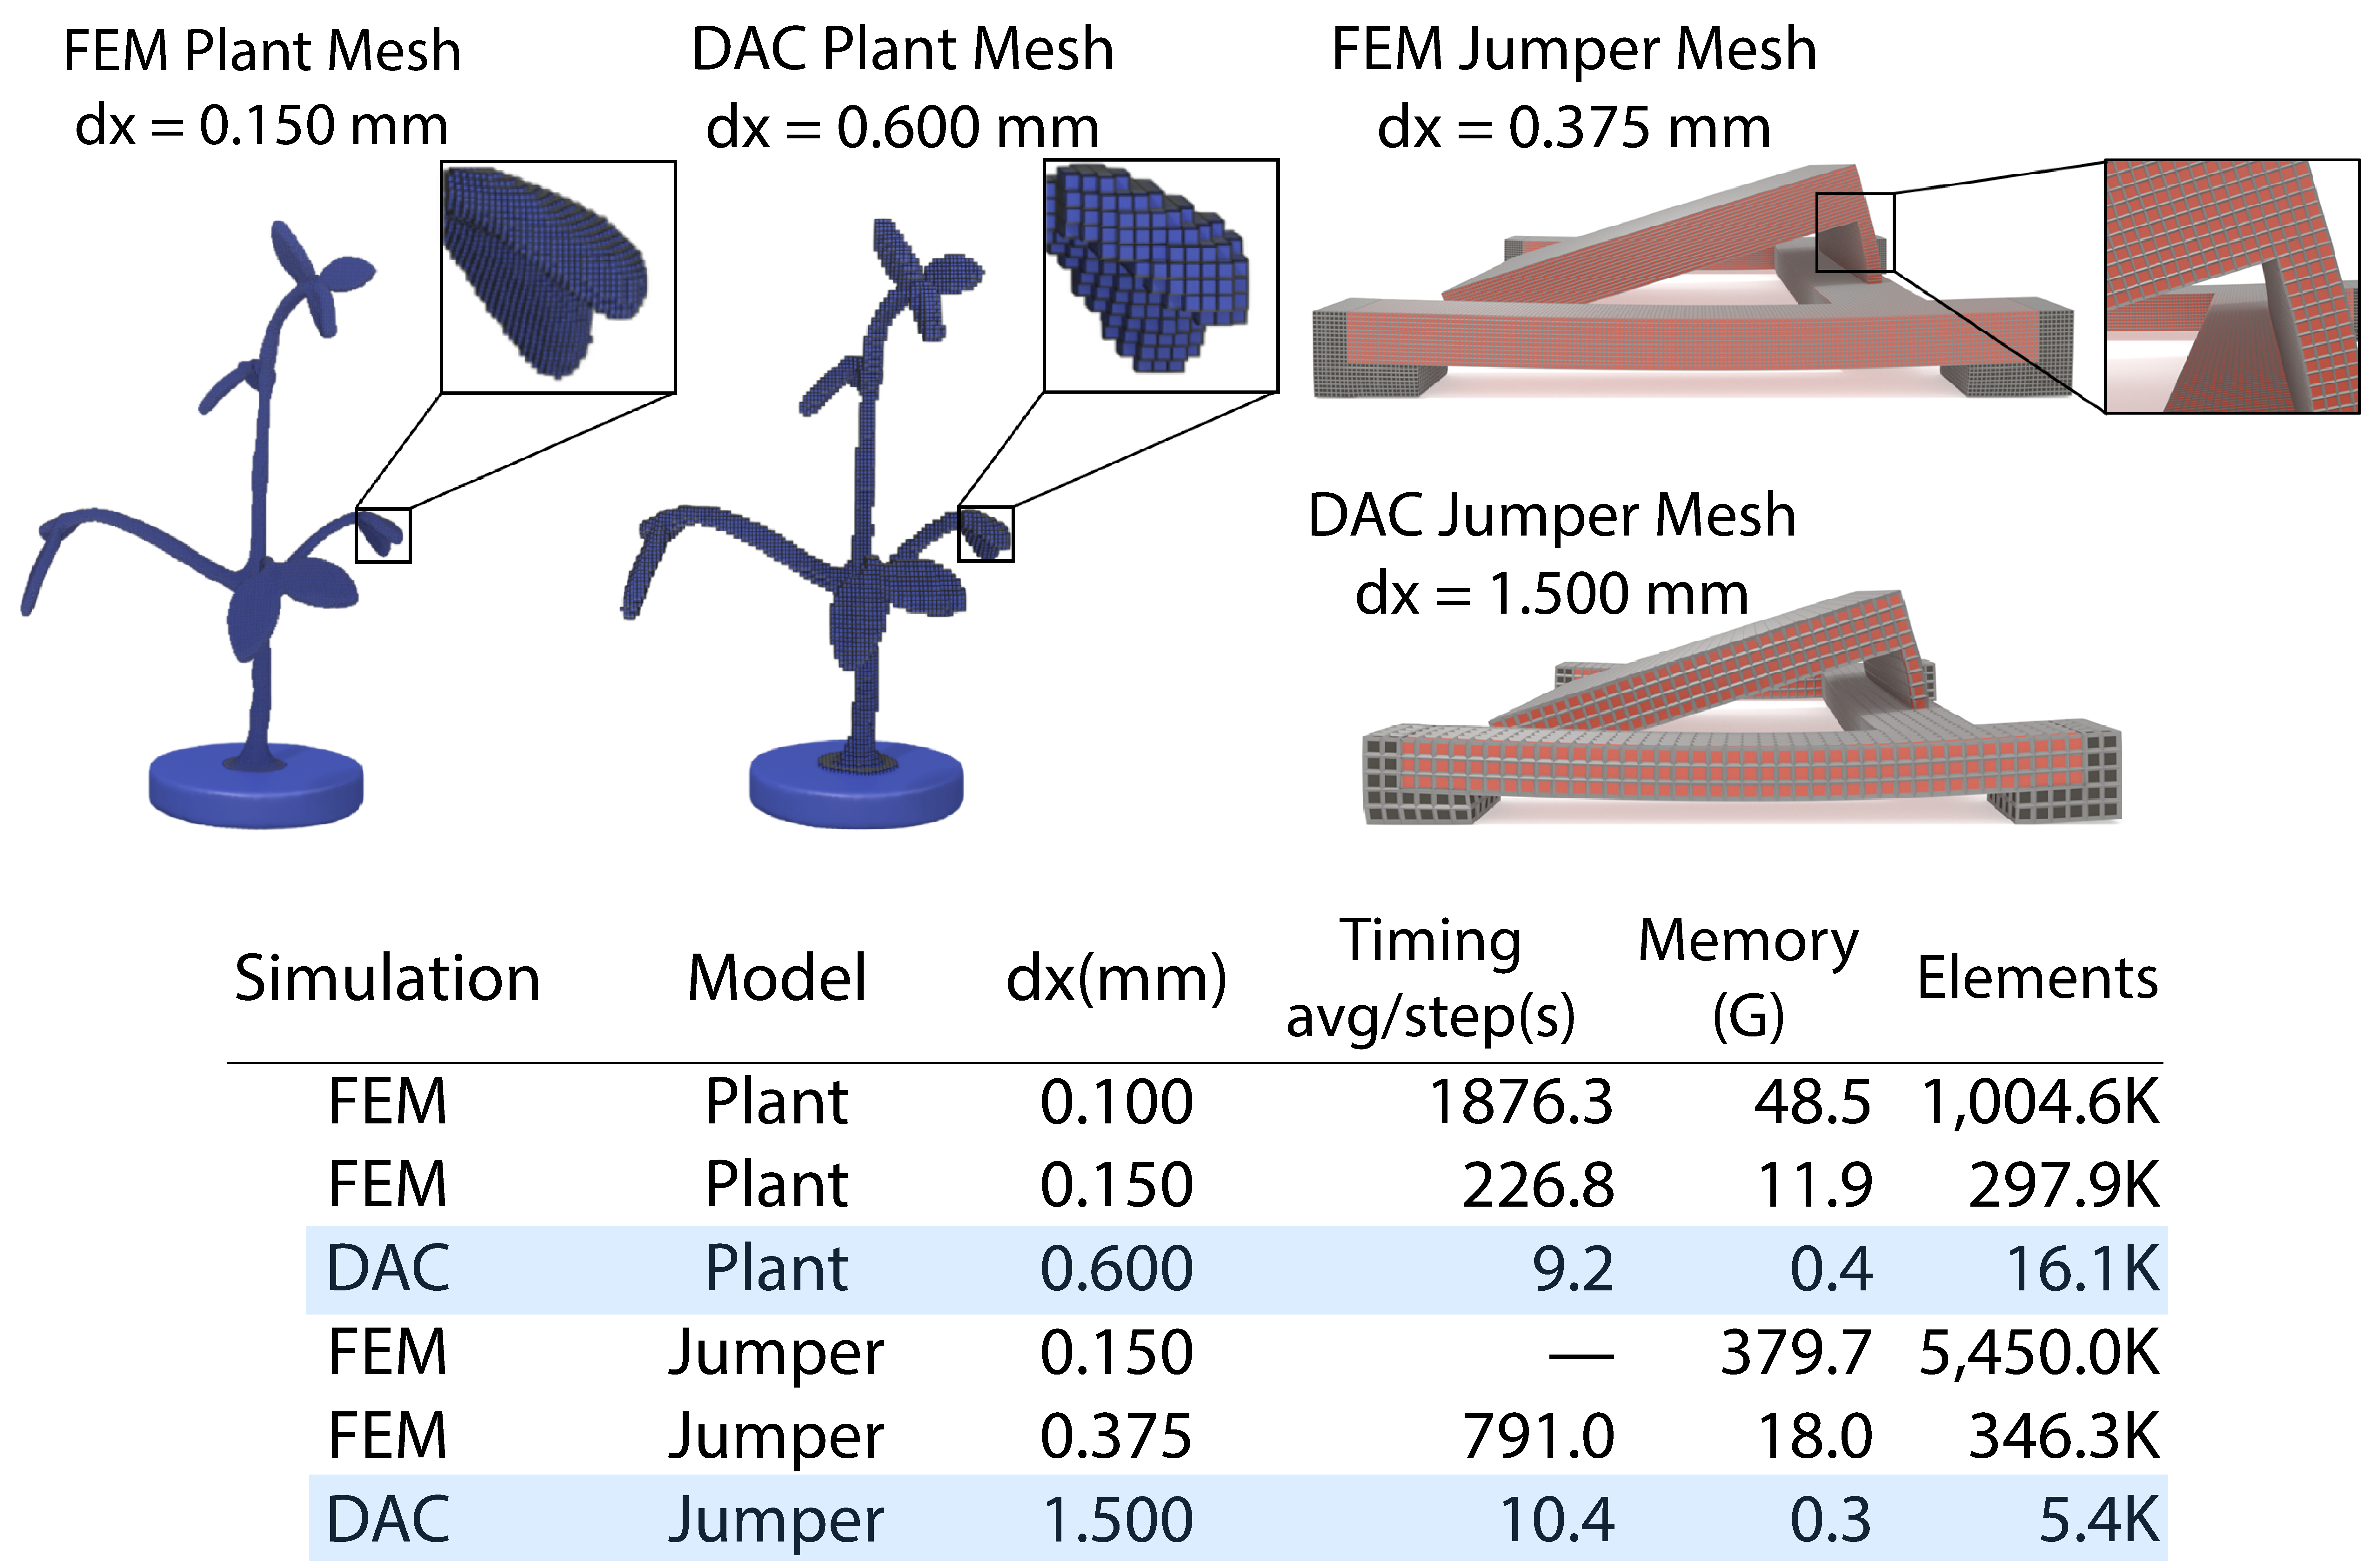
\includegraphics[width=0.8\textwidth]{figs/coarsening_runtime_sim}
	\centering
	\caption{Statistics for our DAC simulations compared with two choices of accurate FE: a convergent FE model, 
		and a validated accurate FE model (validated as matching experimental behavior and modal frequencies are within $5\%$ of convergent values). For each simulation we report the model used (plant and jumper models), the mesh element size,  the average wall-clock time spent per dynamic time step, memory usage, and the number of elements in the simulated mesh. Timings were recorded on an Intel Xeon E5-2666 v3, 2.9Ghz with 4 CPU threads.
	}
	\label{table:suff}
\end{figure}
\section{Boundary Balancing Impact Model}
\label{sec:BBI}

\begin{figure}[h!]
	\centering
	\includegraphics[width=0.8\columnwidth]{images/BBI_jumper_drop.png}
	\caption{Impact model testing with a 3D-printed jumper dropped onto the ground. We show overlaid frames captured, left to right, from an experiment (left) and two corresponding simulations (at $h=10^{-4}s$) that respectively apply DKE (middle) and BBI (right) impact models. In experiment the fabricated jumper lands, bounces up and then rests upright on its feet (left). However, simulation with the DKE model (middle) rebounds too high, flips over and so incorrectly predicts that the jumper will fail by landing on its back after collision (middle). With our BBI model (right), our simulation qualitatively predicts the experimentally determined landing behavior for this design.}
	\label{fig:collision_exp}
\end{figure}

With our DAC discretization in place, we will now derive a new, Boundary-Balancing Impact (BBI) model for FE that gains us accurate prediction of impact-response for the 3D-printed elastic materials we focus on in this work.

\subsection{Complementarity Integration Revisited} 
The nonsmooth Newmark complementarity integrator we reviewed in Section~\ref{sec:simPrelim} has several well-known flaws~\cite{Deuflhard:2008fu} that we illustrate next. In Figure~\ref{fig:BBI_block_compare_all} right, we drop a 3D-printed block from height of 3 cm onto a flat surface. As it is both stiff and highly damped it lands without perceptible rebound. Yet, when we simulate the same drop of the block with the Newmark complementarity integrator the block rebounds up to a height of 0.89 cm; see Figure~\ref{fig:BBI_block_compare_all} left. Errors on this scale are unacceptable in a fabrication design process where they can make the difference between success and failure - see Figure~\ref{fig:collision_exp}.

What is going wrong in these examples? The Newmark discrete velocity update step in (\ref{eq:newmark_free_update}) gives rise to an arbitrary, undesirable (and for elastic materials) generally incorrect choice of restitution. Consider the impact of our material at contact with a normal $\vc n$. Here the complementarity constraints ensure that the new displacement $\delta^{t+1}$ along this normal are zero so that $\vc n^T \delta^{t+1} = 0$. However, although this nicely satisfies position constraints, upon substitution we see that $\vc n^T \vc v^{t+1} =  -\vc n^T \vc v^t$ so that Newmark gives an incorrect, fully elastic (coefficient of restitution $= 1$) effective impact response. Yet the impact response for elastica along an impact boundary should instead be inelastic with the normal velocity on impact along the elastic boundary dissipated completely~\cite{Doyen:2011gka}. In turn this results in much too large rebounds upon impact as we observe in Figures~\ref{fig:collision_exp} and \ref{fig:BBI_block_compare_all}. A related error for complementarity integrators manifests in commonly observed spurious oscillations in positions and tractions along contact boundaries. These oscillations are the combined result of instabilities in contact stresses, velocities and displacements. Notably, both of these issues arise with arbitrary impact geometries, not just in the planar example discussed here.

\subsection{DKE Contact Stabilization} 
To address these widely reported problems,~\citet{Deuflhard:2008fu} introduced a contact stabilization step to filter contact response with projection. They observe that contact forces acting on the material boundary should be balanced and so proposed a now-standard FEM contact-stabilization filter (DKE) that applies an L2-projection that zeroes out normal displacements along the boundary of materials at contact interfaces.  

This projection on displacement is performed at the end of each time step, after the position update (\ref{eq:newmark_contact_implicit}) has been solved. This ensures a correct \emph{inelastic} response at the contact boundary and is effective in producing desirably stabilized contact tractions~\cite{Deuflhard:2008fu,Krause:2012im}. 
Nevertheless, when we compare DKE against experiment (Figures~\ref{fig:collision_exp}, \ref{fig:BBI_block_compare_all}, and \ref{fig:BBI_block_compare_plant}), we see that the DKE projection likewise introduces unacceptably large rebound errors when compared with real-world results.

\begin{figure}
	\centering
	\includegraphics[width=0.8\columnwidth]{images/BBICubeCmp.png}	
	\caption{Impact validation test. A 3D-printed, stiff elastic block is dropped face-first on the ground. Left-to-right we compare the simulated results of three FE impact models  - complementarity, DKE and our BBI model - with experimental results. We show configuration, at start, impact, and post impact maximum rebound height with details on stress distribution at impact, apex height reached, and (inset) the velocity profile for each simulation. As the effective restitution of elastica varies with angle of impact, see below in Figure~\ref{fig:cube_corner} for a comparable oblique drop experiment.}
	\label{fig:BBI_block_compare_all}
\end{figure}

\begin{figure}
	\centering
	\includegraphics[width=0.6\columnwidth]{images/cubeDropCorner.png}	
	\caption{Comparison of our BBI model to experiment for a 3D-printed cube dropped from an oblique initial orientation.}
	\label{fig:cube_corner}
\end{figure}

\subsection{Boundary Balancing Impact}
To better understand why DKE projection does such a poor job of resolving impacts in our elastic materials, let us consider again our simple dropped block example in Figure~\ref{fig:BBI_block_compare_all}.
We observe that by projecting out just the normal component of displacement along the boundary the DKE method artificially \emph{concentrates} high stresses along the elements just inside the boundary. This can be seen in the impact row of Figure~\ref{fig:BBI_block_compare_all}.
These concentrated stresses effectively load the near-boundary layers which then spring back, introducing a much too large response as seen in the final row of Figure~\ref{fig:BBI_block_compare_all}.
The problem here is that the L2-projection applied is material-oblivious and yet material properties clearly mediate impact response. Compliance distributes contact stresses quickly through an elastic material while, in damped materials, internal friction rapidly attenuates the response. 

With these observations in mind we define a new Boundary Balancing Impact (BBI) model that can effectively impose boundary force-balance in a material-aware fashion. Starting with our base time integrator we define a compliant, discretization- and material-aware metric for projection below. The resulting stabilizing impact model better duplicates results in our design applications and experiments. Upon completing each time step from $t-1$ to $t$ we replace the Newmark update in (\ref{eq:newmark_free_update}) with a compliant boundary projection update
\begin{align}
\begin{split}
\vc c &= 2 \vc \delta^{t+1} - h \vc v^t, \\
\vc A &= \vc M + \frac{h^2}{4} \vc K(\vc q^{t+1}) + \frac{h}{2} \vc D(\vc q^{t+1}) ,\\
\vc d^* &= \argmin_{\vc d} \big\{ \frac{1}{2} \| \vc d - \vc c \|^2_{\vc A} : \vc N^T \vc d \geq 0 \big\},\\
\vc v^{t+1} &= \frac{1}{h} \vc d^*,\\
\vc q^{t+1} &= \vc q^t + \vc \delta^{t+1}.\\
\end{split}
\label{eq:newmark_predictor_proj}
\end{align}

This new impact model projects the explicit predicted velocity displacement, $\vc c$, to the nearest set satisfying force balance on the boundary with respect to the local approximation of both material \emph{stiffness} and \emph{damping}. We find that this effectively distributes the contact-stabilized displacement across the material from the boundary layers. The effect of impact is communicated to the material interior while still ensuring that impacts are correctly inelastic along the active contact boundary.
This leads to accurate predictions of real-world bouncing and rebounds. In our simple drop test we see in the impact row of Figure~\ref{fig:BBI_block_compare_all} that, at impact, response for this damped material has been correctly dissipated and the resulting normal displacement closely matches real world results in the apex row of Figure~\ref{fig:BBI_block_compare_all}. 

As we consider a range of impact angles, as well as impact with more complex geometries, multi-material 3D-prints and self contact we see that BBI still consistently and more accurately captures impact-response behavior. See Figures ~\ref{fig:collision_exp}-\ref{fig:flamingo_contact}. These examples demonstrate the range and complexity of responses obtained by BBI coupling impact to stiff elastic materials with large deformations as well as objects composed of multiple materials undergoing both self-contact and stiction.

\begin{figure}
	\centering
	\includegraphics[width=0.8\columnwidth]{images/plantDrop.png}	
	\caption{A drop test of the 3D-printed plant model (digital material). We compare simulated results from Complementarity, DKE and our BBI model with experiment. BBI solely reproduces the observed impact behavior.}
	\label{fig:BBI_block_compare_plant}
\end{figure}

\begin{figure}
	\centering
	\includegraphics[width=\columnwidth]{images/FlamingoDrop.png}	
	\caption{Drop tests of a multi-material 3D-printed flamingo model (Rigur and TangoBlackPlus) from a variety of orientations. While effective restitution of elastica varies with angle of impact, in all cases our BBI simulations agree with experiment.}
	\label{fig:flamingo_contact}
	\vspace{-10px}
\end{figure}
\section{Results and Discussion}
\label{sec:results}

To test our proposed algorithms we compare simulated results generated by DAC and BBI with real-world results experimentally obtained from a range of compliant 3D-printed jumping and throwing mechanisms.
For each mechanism we begin with a dynamic, time-varying goal, e.g., for our \emph{jump-over} goal: ``when pressed and released, jump over a given wall and land upright on the far side'' (see Figure~\ref{fig:over}).

Simulations suitable for fabrication design must accurately predict both when a design fails and when it succeeds, thus we require real world examples of each. Below we outline our approach to creating these mechanism examples for testing, discuss our identification results, and review our implementation. We then detail our experiments comparing DAC and BBI's simulated predictions for each design task below in \S\ref{sec:exp} and validate outcomes of the simulations against repeated user trials in a study discussed in \S\ref{sec:user}.

\subsection{Creating Mechanism Examples} We focus our tests here on jumping-related mechanisms. The analysis and design of jumping mechanisms is an increasingly active~\cite{Anonymous:gFJEnD-w,bergbreiter2007design,Bingham:orient,Bergbreiter:2008te,Jung:2014fh,JeSungKoh:2013ga,Koh:2015cy,Vella:2015cw,ShuguangLi:2015kl}, challenging and practical domain that incorporates high-speed transient dynamics of stiff elastic materials undergoing impact and so is an ideal test case for DAC and BBI.
Research in jumping mechanisms has focused on efficient energy transfer into jump height, see e.g.,~\citet{MinkyunNoh:2012fv}
with aligned research on a range of approaches for controlled jumping~\citep{Loepfe:2015ir,Bartlett:2015he,ShuguangLi:2015kl}. In all cases, to our knowledge, mechanisms have been developed via costly, manual iterations of hands-on experiment, re-design, fabrication and one-off simulations~\citep{Cho:2009jl,Bartlett:2015he}, while even the stable landing of dynamic jumps has remained highly challenging~\citep{Jung:2015gm}.

For each of our jumping and throwing goals (see \S\ref{sec:exp} below) we first attempted to manually create successful designs. We obtained designs that came close to ideal, but, consistent with the above cited literature, we were unable to hand tune these mechanisms to fully satisfy design goals. E.g., for the jump-over goal we found a design that often cleared the wall but did not land upright; see Figure~\ref{fig:over}, left. These mechanisms are our \emph{initial} designs.

Presuming our initial designs are potentially close to successful designs, we perform local optimization over a pair of key design parameters, here generally length and height (see Figure~\ref{fig:params}), to seek a nearby solution. For each mechanism we pose its design goal as an objective and a set of constraints; these functions are detailed in Figure~\ref{table:perf}. To evaluate these objectives and constraints we apply DAC and BBI simulation at each design sample queried by the optimizer. Statistics for the numbers of simulation samples, iterations and timings for performing these local optimizations are summarized in Figure~\ref{table:perf}.

For all these examples we found that a relatively small number of iterations were needed to find successful designs;  this suggests that our initial, hand-tuned designs are close to solutions in a basin. However, practical design optimization would demand a global optimization strategy to resolve non-convexity. In such general cases initial designs can be expected to start far from optima while the search space is often large - local optimization would be insufficient.

The mechanisms found by this process are our \emph{final} designs. We compare the trajectories and outcomes predicted by BBI and DAC against the real world initial and final mechanisms: validation results are detailed for each example below in \S\ref{sec:exp}, while our user study results are presented in \S\ref{sec:user}. The uncut video footage of all experiments are available online~\cite{Video}.

\begin{figure}[h]
	\centering
\includegraphics[width=0.7\columnwidth]{figs/optTable.pdf}
\caption{Design optimization statistics. For each dynamic design optimization we report the design task objectives and constraints applied, the number of optimization iterations performed, the total number of simulations performed for each design and finally the total wall-clock time (minutes) spent in design optimization. Sampled frames for each simulated and corresponding fabricated mechanism designs are given in Figures~\ref{fig:flipper}--\ref{fig:more_flippers} and design parameters optimized over are summarized in Figure~\ref{fig:params}. Here $\theta_c$ and $\vc{x}_c$ represent jumper angle of rotation and catapult projectile center-of-mass position at landing while $\vc{x}_{\text{target}}$ is the desired projectile target.
}
\label{table:perf}	
\end{figure}

\begin{figure}[h!]
\centering
\includegraphics[width=0.7\textwidth]{figs/param.pdf}
\caption{Design geometries and parameters.}
\label{fig:params}
\end{figure}	

\subsection{Implementation}

All results are computed on an Amazon EC2 compute-optimized instance with 4 CPU threads (Intel Xeon E5-2666 v3, 2.9Ghz), while all mechanisms were printed on a Objet500.
While DAC and BBI give us orders of magnitude speedups for predictive simulation of deforming dynamics, our experiments (see Supplemental) show that dynamic FE simulation is unnecessary when modeling initial loading as well as during some portions of free-flight. With careful book-keeping and mapping of state simpler and more efficient models can be employed during these phases to gain further speedup.
When initially loading mechanisms, e.g., when pressing down a jumper in Figure~\ref{fig:simulationStage}, we observe that the process is effectively quasistatic and so simulate with an efficient quasistatic solver detailed in our Supplemental. Upon completion of the initial loading we map state to our full dynamic solver with DAC and BBI.
We also track the time-varying elastic potential energy stored in simulated compliant objects. When damping causes this internal potential to fall to zero, e.g., during portions of free-flight, we switch from our full DAC discretization to a rigid body discretization. We use DMV~\cite{Moser:1991dl}, an efficient energy--momentum preserving rigid-body integrator, to then time step the system in SE(3) coordinates until the next collision is reached, at which point we map rigid-body state back to the DAC model to capture the new deformation dynamics at impact. See our Supplemental for details on this process.

\subsection{Identification}
\begin{figure}[h!]
\centering
\includegraphics[width=0.6\textwidth]{figs/materials_table}
\caption{Material parameters identified by our fine and coarse matching against calibration. Left to right we list previously reported Young's moduli for vertically and horizontally oriented prints compared with our identified moduli. We then report the matched numerical moduli we use for each for our DAC models and finally, list previously unreported damping parameters we identify and use in our simulations. 
}
\label{fig:identified_params}
\end{figure}

We compute each DAC model's coarse mesh resolution and material parameters using the measurement procedure described above in \S\ref{sec:DAC}; see also Figure~\ref{fig:vibration_match}. We model heterogeneous materials by computing numerical Young's moduli for soft (TangoBlackPlus) and rigid (Rigur RGD450) materials and coarsening as much as possible while retaining a single material per element. A major benefit of our coarsening scheme is that it identifies both actual and numerical moduli and damping parameters of real-world materials. Figure \ref{fig:identified_params} details these parameters. The damping parameters we present here have not, to our knowledge, been previously identified in the literature. On the other hand, in our experiments and simulations we find that the previously identified Poisson's ratio for our printed materials~\cite{major2011}, at $0.45$, is effective, and keep it fixed at this value for all examples reported here.
\begin{figure}
	\centering
\includegraphics[width=0.6\textwidth]{figs/measure.pdf}
\caption{Measured and simulated vibrations of a 3D-printed jumper (Rigur) model (magnify the plot for details of fit).}
\label{fig:vibration_match}
\end{figure}

\subsection{Experiments}
\label{sec:exp}

In this section we detail the individual design examples. We visually compare the trajectory behavior of both the real world fabricated initial and final mechanisms with corresponding DAC and BBI simulation results at the same parameters.
In the following section we then discuss the results of the user study we perform to evaluate the results of initial and final fabricated mechanisms over repeated user trials comparing against DAC and BBI predicted simulation outcomes.

\begin{figure}[h!]
	\centering
\includegraphics[width=0.7\columnwidth]{images/ResultsFlipper.png}
\caption{A comparison of experimental (bottom) and DAC/BBI simulated (top) results for initial (left) and final (right) designs of a flipping mechanism.}
\label{fig:flipper}	
\end{figure}

\paragraph{Flipper}
Our first design example is a simple forward flipping jumper. We begin with the geometry in Figure~\ref{fig:flipper} left, load the jumping model by pressing down and then releasing. The design goal is a shape that, upon release, jumps forward into the air, flips and then lands stably on its feet, see e.g., Figure~\ref{fig:simulationStage}. 
See Figure~\ref{fig:flipper} comparing simulated and experimental trajectories for both initial and final design samples.

\begin{figure}[h!]
	\centering
\includegraphics[width=0.7\columnwidth]{./images/ResultsCatapult.png}
\caption{A comparison of experimental (bottom) and DAC/BBI simulated (top) results for initial (left) and final (right) designs of the catapult mechanism.}
\label{fig:catapult}	
\end{figure}

\paragraph{Catapult}
Our next design example is a catapult mechanism. By adding a firing basket to the above flipper geometry, fixing the mechanism base to the ground, and then adding a projectile cube in the basket to the design model we obtain a catapult for throwing metal cubes at targets. This system requires modeling the sliding contact and impact between the cube and basket. The design goal here is to find a catapult geometry that, under loading produces the correct combination of launch position and release velocity for the catapult arm and block so that the block hits a predetermined target. 
See Figure~\ref{fig:catapult} comparing simulated and experimental trajectories for both initial and final design samples.

\begin{figure}[h!]
	\centering
\includegraphics[width=0.7\columnwidth]{./figs/ResultsOnto.pdf}
\caption{A comparison of experimental (bottom) and DAC/BBI simulated (top) results for initial (left) and final (right) designs for a jumper mechanism to jump onto a platform and land upright.}
\label{fig:onto}	
\end{figure}

\paragraph{Jumping onto obstacles}
Here we consider a design example where the goal is  
to find a geometry for a 3D-printed jumper mechanism that, upon release, jumps forward and upwards into the air, flips (possibly multiple times) and then lands stably upon its feet on top of a flat obstacle, see e.g., Figure~\ref{fig:onto}. 
See Figure~\ref{fig:onto} comparing simulated and experimental trajectories for both initial and final design samples.

\begin{figure}[h!]
	\centering
\includegraphics[width=0.7\columnwidth]{./figs/ResultsOver.pdf}
\caption{A comparison of experimental (bottom) and DAC/BBI simulated (top) results for initial (left) and final (right) designs for a jumper mechanism to jump over a wall of specified height and land upright.}
\label{fig:over}	
\end{figure}

\paragraph{Jumping over obstacles}
In this example, the goal is to find a geometry for a 3D-printed mechanism that, upon release, jumps forward and upwards high enough into the air to clear a wall, flip (possibly multiple times) over it and then land stably on the other side. 
See Figure~\ref{fig:over} comparing simulated and experimental trajectories for both initial and final design samples.

\begin{figure}[h!]
	\centering
\includegraphics[width=0.7\columnwidth]{./images/ResultsAllFlippers.png}
\caption{A comparison of experimental (bottom) and DAC/BBI simulated (top) results for six more design samples: initial (left) and final (right) designs of variations on the flipping mechanism (``Normal'').}
\label{fig:more_flippers}	
\end{figure}

\paragraph{Flipper variations}
We additionally evaluate six further design example comparisons between fabricated mechanisms and DAC and BBI simulated trajectories over a range of flipper mechanism variations. In Figure~\ref{fig:more_flippers} we compare initial and final designs created by three variations away form the base initial (``normal'') flipper mechanism design.

\subsection{User Study Results}
\label{sec:user}
Here we present the results of a user study evaluating the goal outcomes of initial and final fabricated mechanisms over repeated user trials as compared against outcomes predicted by DAC and BBI.

\begin{figure}[h!]
\centering
\includegraphics[width=0.7\columnwidth]{./figs/UserStudyCatapult.pdf}
\caption{Statistics summarizing our user study comparing results from trials with our initial and final \emph{catapult} mechanisms. We report the distance to target per trial. The final catapult design dramatically outperforms its initial counterpart, consistently, across all users, coming close to matching DAC/BBI predicted outcomes.}
\label{fig:userStudyCatapult}
\end{figure}

\begin{figure*}[hpt!]
\centering
\includegraphics[width=0.95\textwidth]{./figs/UserStudyJumpers.pdf}
\caption{
Statistics summarizing our user studies comparing results from trials (left to right) with our our initial and final  \emph{flipper}, \emph{jump-onto}, and \emph{jump-over} mechanisms. In orange bars we report the number of successes per user, while in grey we report total successes per mechanism across all trials. Note that  initial designs for both the \emph{jump-onto} and \emph{jump-over} have no successes at all, while, across all three mechanisms, final designs dramatically outperform their initial counterparts. This success is consistent across all users - closely matching DAC/BBI predicted outcomes.}
\label{fig:userStudyJumpers}
\end{figure*}

We asked five users to perform twenty attempts each with both the initial and final versions of each of the above mechanisms; the flipper, catapult, jump onto and jump over. For the flipper, jump onto and jump over mechanisms we count the number of successful attempts for each user; see Figure~\ref{fig:userStudyJumpers}. Here we define goal success as satisfying the objectives and constraints posed by each design as described above; e.g. flipping, clearing all obstacles, and landing feet down on the desired area (Figures \ref{fig:flipper}, \ref{fig:onto} and \ref{fig:over}).
In Figure~\ref{fig:userStudyJumpers} we summarize the total number of successes for each user per optimized and unoptimized design as well as the aggregate totals. For the optimized and unoptimized catapult designs we report the mean distance to the target in millimeters and the standard deviation for each user~(\autoref{fig:userStudyCatapult}). 

In order to consistently apply the loading force to each mechanism, users are instructed to fully load each mechanisms by pressing the top until it makes contact with the bottom. We ask users to apply the loading force with a 3D printed bar at a designated loading point marked on each mechanism with permanent marker. The user then deformed the mechanism to the loaded state and released the load with a sliding motion, similar to the launching motion in Tiddlywinks. This ensures that contact break between the stick and the mechanism is close-to instantaneous and consistent.  The same criteria are used in simulation to obtain comparable loading. The Objet500 we employ in all our fabrication examples works at 85 microns precision while our design parameter changes are on the order of millimeters and are thus be reliably manufactured. Additionally to further  minimize variability in experimental conditions we use the same printer for all examples and always print in the top left area of the build tray. We orient models consistently and perform experiments within two weeks of printing to avoid long-term material degradation - an interesting topic for future modeling and design research.

Throughout the study, mechanism goal outcomes consistently matched those predicted by their corresponding DAC/BBI simulations. Final, optimized, mechanisms were much more reliable than their initial counterparts - under simulation these were successful. In terms of jumping (flipping, over, onto) tasks final designs completed more than $85\%$ of their attempts for every task - close to matching DAC/BBI predicted success. while the initial designs successfully completed the simplest flipping task in $3\%$ of all attempts~(\autoref{fig:userStudyJumpers}) and had zero successes for the jump-onto and jump-over tasks - matching DAC/BBI predicted failure. This large difference validates that designed mechanism successes are quite reliably modeled by DAC/BBI.
For instance, our catapult design achieves a $10\times$ reduction in mean error with respect to target distance for all users. Note that here there is a small increase in standard deviation due to the fact that our optimized design of the catapult necessarily throws the cube much further, amplifying any variation errors in initial targeting~(\autoref{fig:userStudyCatapult}).
For supporting evidence of each mechanism's experimental behavior please see our supplemental materials which include uncut videos~\cite{Video} of all user studies.
\include{Conclusion}
\appendix
\include{appa}
\chapter{Implementation and Additional Experiments for Dynamics}
\section{Dynamic Contact-Impact Solver}
\label{sec:iter_dyn_solver}
\paragraph{Implicit time stepping method} 
At each time step our implicit contact method must jointly satisfy the discrete equations of motion
%
\begin{align}
\begin{split}
\vc M \vc \delta^{t+1} & - \vc b^t - \tfrac{h^2}{4} \vc F(\vc q^{t+1}) + \tfrac{h^2}{4} \vc D(\vc q^{t+1}) \vc v^{t+1} \\
&- \tfrac{h^2}{2} \vc N \alpha -  \tfrac{h^2}{2}  \vc T \beta = 0, 
\label{eq:ap_newmark_contact_implicit}
\end{split}
\end{align}
updates
\begin{align}
\begin{split}
\vc b^t &= h \vc M \vc v^t + \tfrac{h^2}{4} \vc F( \vc q^t) -\tfrac{h^2}{4} \vc D( \vc q^t) \vc v^t, \\
\vc q^{t+1} &= \vc q^t + \vc \delta^{t+1},
\end{split}
\end{align}
%
contact conditions\footnote{$\vc x \perp \vc y$ is the \emph{complementarity condition} $\vc x_i \vc y_i = 0,\ \forall i$.} 
%
\begin{align}
0 \leq \alpha \perp \vc N^T \delta^{t+1} \geq 0, 
\label{eq:ap_contact_conditions}
\end{align}
%
variational maximal dissipation conditions
%
\begin{align}
\begin{split}
\min_{\beta} \{ \beta^T \vc T^T (\tfrac{2}{h} \delta^{t+1} - \vc v^t) : \mu_k \bar{\alpha}_k \geq \|\bar{\beta}_k\|, \> \forall k \in \mathcal{C} \}, 
\label{eq:ap_max_diss_transform}
\end{split}
\end{align} 
%
and the impact projection
%
\begin{align}
\begin{split}
\vc c &= 2 \vc \delta^{t+1} - h \vc v^t, \\
\vc A &= \vc M + \frac{h^2}{4} \vc K(\vc q^{t+1}) + \frac{h}{2} \vc D(\vc q^{t+1}) ,\\
\vc d^* &= \argmin_{\vc d} \big\{ \| \vc d - \vc c \|^2_{\vc A} : \vc N^T \vc d \geq 0 \big\},\\
\vc v^{t+1} &= \frac{1}{h} \vc d^*,\\
\end{split}
\label{eq:ap_newmark_predictor_proj}
\end{align}
to convergence with an iterative solver.

\paragraph*{Modified Newton-Raphson with frictional contact}
To construct our solver we first consider time-stepping without contact forces. At each time step we seek a displacement update $\delta^{t+1}$ satisfying 
\begin{align}
\vc f(\delta^{t+1}) = \vc M \delta^{t+1} - \vc b^t - \tfrac{h^2}{4} \vc F(\vc q^{t+1}) + \tfrac{h^2}{4}  \vc D(\vc q^{t+1}) \vc v^{t+1}=0,
\end{align}
%
with 
\begin{align}
\begin{split}
\vc q^{t+1} &= \vc q^t + \vc \delta^{t+1},\\
\vc v^{t+1} &= \tfrac{2}{h} \vc \delta^{t+1} - \vc v^t.
\end{split}
\end{align}
%
Ignoring $\frac{\partial \vc D}{\partial \vc q}$ we set
\begin{align}
\vc H(\delta)  = \vc M + \frac{h^2}{4} \vc K(\vc q^t + \delta) + \frac{h}{2} \vc D(\vc q^t + \delta).
\end{align}
and have $\nabla \vc f \simeq \vc H$. In the following we will reserve superscripting with indexing $t$ for time step increments and superscripting with indexing $i$ for iteration increments. Modified Newton-Raphson then approximates the linearization of $\vc f$, at iterate $i$, around $\delta^i$
as 
\begin{align}
\vc f(\delta^{i+1}) \simeq   \vc f(\delta^i) + \vc H(\delta^i) (\delta^{i+1} - \delta^{i}).
\end{align}
We then find the improved estimate of displacement $\delta^{i+1}$ by line search on the descent direction
\begin{align}
\delta^{i} - \vc H(\delta^i)^{-1} \vc f(\delta^i).
\end{align}
%as a descent direction for line search to obtain a final $\delta_{i+1}$.
%We apply a line search by bi-section to avoid instability of Newton's method.

With contact, at each Newton iterate we are now solving for updated triples of both displacement and boundary contact and friction forces, $(\delta, \vc \alpha, \vc \beta)$. 
Applying the same modified linearization of (\ref{eq:ap_newmark_contact_implicit}) about $\delta^{i-1}$ then gives 
\begin{align}
\vc f(\delta^{i-1}) + \vc H(\delta^{i-1}) (\delta^i - \delta^{i-1}) - \tfrac{h^2}{2} \vc N \alpha -  \tfrac{h^2}{2}  \vc T \beta = 0,
\end{align}
Setting 
\begin{align}
\begin{split}
%\vc r(\delta) &=  \vc b^t + \tfrac{h^2}{4} \vc F(\vc q^{t} + \delta) + \tfrac{h^2}{4} \vc D(\vc q^{t} + \delta) (2\delta - \vc v^{t}) \\
%& -  \big[ \frac{h^2}{4} \vc K(\vc q^{t}+\delta) + \frac{h}{2} \vc D(\vc q^{t} + \delta) \big] \delta 
\vc r(\delta) &=  \vc b^t + \tfrac{h^2}{4} \vc F(\vc q^{t} + \delta) - \tfrac{h^2}{4} \vc D(\vc q^{t} + \delta) (\frac{2}{h}\delta - \vc v^{t}) \\
& +  \big[ \frac{h^2}{4} \vc K(\vc q^{t}+\delta) + \frac{h}{2} \vc D(\vc q^{t} + \delta) \big] \delta 
\end{split}
\end{align}
at each Newton iterate, the linearized contacting system we want to solve is then 
\begin{align}
\begin{split}
& \vc H(\delta^{i-1}) \delta^i =  \vc r(\delta^{i-1}) + \tfrac{h^2}{2} \vc N \alpha +  \tfrac{h^2}{2}  \vc T \beta,\\
& 0 \leq \lambda \perp \vc N^T \delta_{i+1} \geq 0,\\
& \min_{\beta} \{ \beta^T \vc T^T (\tfrac{2}{h} \delta^{t+1} - \vc v^t) : \mu_k \bar{\alpha}_k \geq \|\bar{\beta}_k\|, \> \forall k \in \mathcal{C} \}
\end{split}
\end{align}
or, equivalently 
\begin{align}
\begin{split}
0 \leq \lambda \perp & \tfrac{h^2}{2} \vc N^T \vc H(\delta^{i-1})^{-1}  \vc N \alpha  \\
&+ \vc N^T \vc H(\delta^{i-1})^{-1} \big[\vc r(\delta^{i-1}) +  \tfrac{h^2}{2}  \vc T \beta \big] \geq 0,\\
\min_{\beta} \{ \beta^T & \vc T^T (\tfrac{2}{h} \delta^{t+1} - \vc v^t) : \mu_k \bar{\alpha}_k \geq \|\bar{\beta}_k\|, \> \forall k \in \mathcal{C} \}
\end{split}
\end{align}
with the update $ \delta^i =  \vc H(\delta^{i-1})^{-1} \big[\vc r(\delta^{i-1}) + \tfrac{h^2}{2} \vc N \alpha +  \tfrac{h^2}{2}  \vc T \beta \big]$.

\paragraph*{Inner-loop solve of Newton steps}
To solve each Newton step we first backsolve to get 
\begin{align}
\begin{split}
&\tilde{\vc N} = \vc H(\delta^{i-1})^{-1}  \vc N, \\
&\tilde{\vc D} =\vc H(\delta^{i-1})^{-1}  \vc D, \\
&\tilde{\vc r} = \vc H(\delta^{i-1})^{-1}  \vc r(\delta^{i-1})
\end{split}
\label{eq:newton_quant}
\end{align}
The solution then simplifies a bit further to finding
\begin{align}
\begin{split}
0 \leq \lambda \perp & \vc N^T \tilde{\vc N} \alpha  + \tilde{\vc N}^T \big[ \tfrac{2}{h^2} \tilde{\vc r} +  \tilde{\vc T} \beta \big] \geq 0,\\
\min_{\beta} \{ \beta^T & \vc T^T  \tilde{\vc T} \beta + \beta^T \vc T^T  \big[ \tilde{\vc N} \alpha  + \tfrac{2}{h^2} \tilde{\vc r} - \tfrac{1}{h} \vc v^t \big] \\
& : \> \mu_k \bar{\alpha}_k \geq \|\bar{\beta}_k\|, \> \forall k \in \mathcal{C} \}.
\label{eq:simple_NCP}
\end{split}
\end{align}
We then solve the Newton step Gauss-Seidel fashion. Each Gauss-Seidel pass  iteratively holds all unknowns except for forces at a single contact $k \in \mathcal{C}$ fixed. We solve for the forces at $k$, update them and then move on to the next $k+1\in \mathcal{C}$. We run multiple Gauss-Seidel passes through the system until convergence is reached satisfying (\ref{eq:simple_NCP}). 

To solve for the updated forces $(\bar{\alpha}_k^{i+1}, \bar{\beta}_k^{i+1})$ for contact $k \in \mathcal{C}$ in Gauss-Seidel pass $i+1$ we compute
\begin{align}
\begin{split}
\vc d_k &=  \sum_{j<k} \tilde{\vc n}_j \alpha_j^{i+1} +  \sum_{j>k} \tilde{\vc n}_j \alpha_j^i \\
& \> \> \> + \sum_{j<k}  \tilde{\vc T}_j \beta_j^{i+1} + \sum_{j>k} \tilde{\vc T}_j \beta_j^i+ \frac{2}{h^2} \tilde{\vc r}_k \in \mathbb{R}^n.
\end{split}
\end{align}
Substituting in (\ref{eq:simple_NCP}) we then solve the single-point frictional-contact problem at contact k. This is just the small, three-dimensional problem to find $(\bar{\alpha}_k^{i+1}, \bar{\beta}_k^{i+1}) \in \mathbb{R}^3$ satisfying
\begin{align}
\begin{split}
0 \leq \bar{\alpha}_k^{i+1} \perp  \vc n_k^T & \tilde{\vc n}_k \bar{\alpha}_k^{i+1}  + \vc n_k^T \tilde{\vc T}_k \bar{\beta}_k^{i+1} + \vc n_k^T \vc d_k \geq 0,\\
\bar{\beta}_k^{i+1} = \argmin_{\bar{\beta}_k} \{ &\bar{\beta}_k \vc T_k^T  \tilde{\vc T}_k \bar{\beta}_k + \bar{\beta}_k \vc T_k^T(\tilde{\vc n}_k \bar{\alpha}_k^{i+1} +   \vc d_k- \tfrac{1}{h} \vc v^t) \\
&  : \> \mu_k \alpha^{i+1}_k \geq \|\bar{\beta}_k\|\}.
\end{split}
\end{align}
We then update to $(\bar{\alpha}_k^{i+1}, \bar{\beta}_k^{i+1})$ and move on to contact $k+1$.

On convergence of this \emph{inner} Gauss-Seidel iteration to optimal $(\alpha^*,\beta^*)$ we update to the next Newton step displacement estimate to
\begin{align}
\delta^i = \tilde{\vc r} + \tfrac{h^2}{2} \tilde{\vc N} \lambda^* + \tfrac{h^2}{2}\tilde{\vc T} \beta^*
\end{align} 
We form the new needed quantities for the next Newton step in (\ref{eq:newton_quant}) and then solve the next Newton step with Gauss-Seidel. On convergence of the \emph{outer} Newton iteration to satisfying (\ref{eq:ap_newmark_contact_implicit}), (\ref{eq:ap_contact_conditions}), and (\ref{eq:ap_max_diss_transform}) we then perform the Impact projection in (\ref{eq:ap_newmark_predictor_proj}) described below and then move to the next time step. 

\paragraph*{Impact model solve}
To solve the BBI impact projection step in (\ref{eq:ap_newmark_predictor_proj}) we can reuse the already computed \emph{final} compliant term from the last iterate in (\ref{eq:newton_quant}). In dual form our BBI impact projection is equivalent to solving the system 
\begin{align}
\begin{split}
0 \leq \lambda \perp & \vc N^T \tilde{\vc N} \lambda  + \tilde{\vc N}^T \vc c \geq 0,\\
\label{eq:impact_proj}
\end{split}
\end{align}
and applying a final velocity update 
\begin{align}
\vc v^{t+1} \leftarrow \frac{1}{h} (\vc c + \tilde{\vc N} \lambda),  
\end{align}
with $\vc c$ given from (\ref{eq:ap_newmark_predictor_proj}). We solve the linear-complementarity problem in (\ref{eq:impact_proj}) with projected Gauss-Seidel. 
\section{SE(3) Projections}

During free-flight motion we can project each body's FE state to a fitted rigid body model equipped with rotational $\vr R \in SO(3)$ and translational $\vr t \in \mathbb{R}^3$ degrees of freedom. Per body we choose coordinates so that $\vr R$ rotates from principal-axis--aligned body frame to world frame and $\vr t$ gives the location of center of mass.
Corresponding angular and linear momenta are $\vr \pi, \> \vr l \in \mathbb{R}^3$, with diagonal inertia tensor $I$ and mass $m$. Nodal positions of material points $\vr x_i$ during rigid motion are then $\vr x^t_i = \vr t^t + \vr R^t (\vr x^0_i - \vr t^0)$. We set corresponding momenta 
to $(\vr p_1^T, ..., \vr p_n^T)^T  = \vc M \vc v^t \in \mathbb{R}^{3n}$, stack nodal vertices as $\vc Q = (\vr x_1, ..., \vr x_n) \in \mathbb{R}^{3 \times n}$ and then project to rigid state with
%
\begin{align}
\begin{split}
\label{eq:FE_to_SE3}
&\vr R^t \leftarrow \argmin_{\vr T \in SO(3)} || \vr T \vc Q^t  - \vc Q^0 ||_F,\\
&\vr \pi^t \leftarrow \sum_{i = 1}^n (\vr x_i^t - \vr t^t) \times \vr p^t_i, \> \>  \> \> \vr l^t \leftarrow \sum_{i= 1}^n \vr p^t_i, \\
%&\vr p^t \leftarrow \sum_x \vr p_x, \\ 
&\vr I  \leftarrow \int_{\Omega^0} \rho(\vr x) [\vr x] [\vr x]^T  dV, \> \> \> \> m  \leftarrow \int_{\Omega^0} \rho(\vr x) dV.
\end{split}
\end{align}

We then timestep rigid body state forward through free-flight with DMV~\cite{Moser:1991dl}, an energy--momentum preserving rigid-body integrator, until the next collision is reached. Upon collision we again need to model elastic behavior and so project back to closest FE state with nodal positions and velocities 

\begin{align}
\begin{split}
&\vr x^t_i \leftarrow \vr t^t + \vr R^t (\vr x^0_i - \vr t^0),\\
&\vr v^t_i \leftarrow \tfrac{1}{m} \vr l^t - \vr R^t (\vr x^0_i - \vr t^0) \times (\vr I^{-1}{\vr \pi}^t).
\end{split}
\end{align}

Comparing the output trajectories between the full FEM simulation and our hybrid projection trajectory we find a tight match throughout.
We show the trajectories obtained from full FEM and the hybrid for our \emph{jumping-over} example. Both simulations are initialized to the same configuration and terminate at first impact. Here the jumper traces out an approximately $20$cm long trajectory while the two simulated trajectories differ in the $L^{\infty}$-norm by $0.63$ mm for the linear trajectory, i.e., center of mass, and $0.02$ radians in rotational pose over the trajectory.
\section{Static Contact Solver}
\label{sec:iter_static_solver}

\paragraph{Loading model}
We observe in experiment that initial loading processes are effectively quasistatic, with no-slip at contacts. We then model the loading phase with a custom static solver that finds equilibrium state subject to satisfying no-penetration contact constraints $\vc p \geq 0$ and an assumption of infinite (no-slip) friction. 
We solve for a $ \delta$ that gives the constrained equilibrium system maximizing frictional work
\begin{align}
\begin{split}
% - \nabla W(\vc q^0 + \delta)  =  F(\vc q^0 + \delta)
F(\vc q^0 + \delta) + \vc N \alpha + \vc T \beta + \vc F_{load} = 0, \\ 
0 \leq \alpha \perp \vc p( \vc q^0 + \delta) \geq 0,\\
%\alpha^T \vc D^T \delta = 0.
\alpha \perp {\vc T}^T \delta, \> \forall k \in \mathcal{C}.
\end{split}
\label{eq:static_var}
\end{align}

\paragraph{Static solver} Our static solver applies a direct solution approach to compute nodal positions $\vc q$ subject to external loads $\vc F_{ext}$ with infinite-friction (no-slip) unilateral breaking contact. 
%requiring $\vc F(\vc q) = \vc F_{ext}$.
At each iteration step $i$, we initialize a Newton-Raphson search direction $\delta^i$ 
\[
\vc K(\vc q^{i})\delta^i = \vc F_{ext} - \vc F(\vc q^{i}).
\]
subject to Dirichlet boundary conditions fixing a set of previously identified \emph{active} contacting boundary vertices identified in the prior iterate. 
At each iteration we apply a projected line search. We first analyze the depth-component of all the previously identified active contacting points $\vc q_{j}$. If $\vc q_{j}$ penetrates an obstacle, we half the step size of the search direction until the penetration depth for that point is less than $10^{-2} \times dx$ where $dx$ is characteristic rest element size in our discretization. After applying the line search, we then update the set of active contacting vertices as follows and take the next iterate step.
Initially, all vertices touching an obstacle boundary are treated as fixed vertices.
We then update the active set of contacting vertices by examining force consistency on all vertices currently contacting the boundary. If the force on a contacting boundary vertex opposes the contacting normal direction, we free it by removing it from the active set; if a contacting boundary vertex was previously free and is now penetrating, we project it back to the contact boundary surface and add it to the active set. We run this solve to convergence satisfying equilibrium in (\ref{eq:static_var}).

We verify our static solver with respect to full dynamic FEM simulation modeling loading with frictional contact. We find that the relative geometric difference between solutions is $0.2\%$ (Hausdorff distance) while the relative difference between
internal energies is $0.4\%$, with an overall 15X speedup gain from the static solver over the dynamic FEM loading simulation.

\section{Stiffness Consistent Mass Matrix}

We assemble our full mass matrix from element mass matrices. Within each element $e$, we integrate
\[
\mathbf{M}_e = \int_{\Omega_e} \sum_{i=1}^8\rho_e \mathbf{N}_i(\xi)\mathbf{N}_i^T(\xi)d\Omega
\]
using 2-point Gauss quadrature.
Here $\mathbf{N}_i$s are the tri-linear shape functions used for our FE calculations including stress computation. Thus the mass matrix is stiffness-consistent and consistently captures both linear and angular momentum of the system.

\section{Constraint assembly}
\label{sec:constraint_assembly}

For each contact $k \in \mathcal C$, the relative acceleration between material points $\vr x_i$ and $\vr x_j$ (at contact $k$) can be expressed via the map $\vc \Gamma_k: \dot{\vc q} \rightarrow \dot{\vr x}_i - \dot{\vr x}_j$. If $\vr y \in \mathbb{R}^3$ is a force applied to point $\vr x_i$, and an equal but opposite force is applied to point $\vr x_j$, $ \vc \Gamma_k ^T \vr y$ is the resulting generalized force applied to the contacting system.
%
For contact $k$, the map $\vc \Gamma_k$ is the sparse matrix with non-zero entries corresponding to nodes participating in the contacting vertex or vertices.
%
For nodal vertex-boundary contact, a single identity entry corresponding to the node's DoFs is sufficient. For vertex-quadrilateral contacts, we compute the signed identity entries for the five participating face node DoFs weighted by the bilinear weights of the contacting points in the face quadrilateral.
\section{Experiments on Choosing Predictive Simulation}
Accurate physical modeling of transient dynamics with contact is validated by experiment and generally requires simulation at close to convergent spatial and temporal grid sizes. This makes even a single forward dynamic simulation run in 3D prohibitively expensive. 
On the other end of the spectrum physically based animation methods seek efficiency by pushing simulations towards maximally stable time-step sizes and coarsest possible spatial meshes to obtain visually appealing but generally highly inaccurate dynamics.
Here we detail our experiments and investigations towards designing predictive and efficient simulation of high-speed dynamics under frictional contact, impact, loading and free-flight suitable for fabrication design.

\include{biblio}
\end{document}

